\documentclass[11pt,a4paper]{article}

% Image mode: pdf.
% Image paths stay relative. In PDF mode, place same-basename PDF conversions
% of the chapter SVG files in the assets/ directory beside this source.

\usepackage{iftex}
\ifPDFTeX
  \PackageError{handout}{This template requires XeTeX or Tectonic}{Compile with xelatex or tectonic.}
\fi

\usepackage[a4paper,top=18mm,bottom=20mm,left=20mm,right=20mm,headsep=6mm]{geometry}
\usepackage{fontspec}
\usepackage{xeCJK}
\usepackage{amsmath}
\usepackage{unicode-math}

% Font settings are intentionally visible in the generated .tex file.
% These defaults target the macOS machine used for the released PDF.
% Change the family names when compiling on another system.
\setmainfont{Songti TC}
\setsansfont{Heiti TC}
\setmonofont{Menlo}
\setCJKmainfont{Songti TC}
\setCJKsansfont{Heiti TC}
\setCJKmonofont{Heiti TC}
\setmathfont{STIX Two Math}
\XeTeXlinebreaklocale "zh"
\XeTeXlinebreakskip=0pt plus 1pt

\usepackage{xcolor}
\definecolor{HandoutBlue}{HTML}{215A91}
\definecolor{HandoutBlueLight}{HTML}{EEF5FC}
\definecolor{HandoutGreen}{HTML}{39715A}
\definecolor{HandoutGreenLight}{HTML}{EFF8F3}
\definecolor{HandoutGold}{HTML}{8A641C}
\definecolor{HandoutGoldLight}{HTML}{FFF8E8}
\definecolor{HandoutInk}{HTML}{253142}
\definecolor{HandoutMuted}{HTML}{667085}

\usepackage{graphicx}
\makeatletter
% Pandoc 3 emits an accessibility `alt` key for raster/PDF images. Older
% graphicx releases do not know that key, so accept it without changing layout.
\@ifundefined{KV@Gin@alt}{\define@key{Gin}{alt}{}}{}
\newsavebox\pandoc@box
\newcommand*\pandocbounded[1]{%
  \sbox\pandoc@box{#1}%
  \Gscale@div\@tempa{\textheight}{\dimexpr\ht\pandoc@box+\dp\pandoc@box\relax}%
  \Gscale@div\@tempb{\linewidth}{\wd\pandoc@box}%
  \ifdim\@tempb\p@<\@tempa\p@\let\@tempa\@tempb\fi
  \ifdim\@tempa\p@<\p@\scalebox{\@tempa}{\usebox\pandoc@box}%
  \else\usebox{\pandoc@box}%
  \fi
}
\makeatother
\usepackage{float}
\floatplacement{figure}{H}
% Pandoc uses LTcaptype=none for uncaptioned longtables. The caption package
% expects that name to exist as a counter even though it is never displayed.
\newcounter{none}
\usepackage{caption}
\captionsetup[figure]{labelformat=empty,labelsep=none,font=small}

\usepackage{booktabs,longtable,array,calc}
\usepackage{etoolbox}
\makeatletter
\patchcmd\longtable{\par}{\if@noskipsec\mbox{}\fi\par}{}{}
\makeatother

\usepackage[most]{tcolorbox}
\tcbuselibrary{breakable,skins}
\newtcolorbox{HandoutLearningMap}{
  enhanced,breakable,colback=HandoutBlueLight,colframe=HandoutBlue,
  boxrule=0.8pt,arc=1.5mm,left=3mm,right=3mm,top=2mm,bottom=2mm,
  before skip=8pt,after skip=10pt
}
\newtcolorbox{HandoutWorkedExample}{
  enhanced,breakable,colback=HandoutGreenLight,colframe=HandoutGreen,
  boxrule=0.65pt,arc=1.5mm,left=3mm,right=3mm,top=2mm,bottom=2mm,
  before skip=8pt,after skip=10pt
}
\newtcolorbox{HandoutSelfCheck}{
  enhanced,breakable,colback=HandoutGoldLight,colframe=HandoutGold,
  boxrule=0.65pt,arc=1.5mm,left=3mm,right=3mm,top=2mm,bottom=2mm,
  before skip=8pt,after skip=10pt
}

\usepackage{titlesec}
\titleformat{\section}{\sffamily\bfseries\Large\color{HandoutBlue}}{}{0pt}{}
\titleformat{\subsection}{\sffamily\bfseries\large\color{HandoutInk}}{}{0pt}{}
\titleformat{\subsubsection}{\sffamily\bfseries\normalsize\color{HandoutInk}}{}{0pt}{}
\titlespacing*{\section}{0pt}{1.4em}{0.55em}
\titlespacing*{\subsection}{0pt}{1.15em}{0.45em}
\titlespacing*{\subsubsection}{0pt}{0.9em}{0.35em}
\setcounter{secnumdepth}{-\maxdimen}

\usepackage{hyperref}
\usepackage{bookmark}
\IfFileExists{xurl.sty}{\usepackage{xurl}}{}
\urlstyle{same}
\hypersetup{
  colorlinks=true,
  linkcolor=HandoutBlue,
  urlcolor=HandoutBlue,
  citecolor=HandoutBlue,
  pdftitle={選化V-2 環境化學},
  pdfsubject={化學},
  pdfcreator={Pandoc with the HighSchooContent LaTeX template}
}

\setlength{\parindent}{0pt}
\setlength{\parskip}{0.55em plus 0.15em minus 0.1em}
\setlength{\emergencystretch}{3em}
\setlength{\LTpre}{0.5em}
\setlength{\LTpost}{0.5em}
\renewcommand{\arraystretch}{1.18}
\providecommand{\tightlist}{%
  \setlength{\itemsep}{0pt}\setlength{\parskip}{0pt}}
\pagestyle{plain}


\begin{document}

\begin{tcolorbox}[
  enhanced,colback=white,colframe=HandoutBlue,boxrule=1.1pt,arc=2mm,
  borderline west={3pt}{0pt}{HandoutBlue},left=5mm,right=4mm,top=4mm,bottom=4mm
]
{\sffamily\small\bfseries\color{HandoutBlue}學生講義}\par
{\sffamily\bfseries\LARGE\color{HandoutInk}選化V-2 環境化學}\par
\vspace{0.35em}{\large 以物料守恆、反應機制與資料尺度，分析污染、資源與能源系統}\par
\vspace{0.45em}{\small\color{HandoutMuted}%
科目：化學
\quad 課程：普通高中選修化學 V
\quad 版本：學生版｜核心＋理解
\quad 校訂：2026-08-29
}\par
\vspace{0.25em}{\small\color{HandoutMuted}範圍：現行選修化學 V 第二章主線；涵蓋綠色化學、科學模型、臭氧層、水與空氣污染檢測、永續發展、氮循環及能源生命週期}\par
\end{tcolorbox}


環境化學研究物質在空氣、水、土壤與生物之間的來源、轉化、傳輸、累積與移除。化學式提供反應機制，濃度與通量描述尺度，科學模型把可量測證據連到尚未直接觀察的過程。本章建立的工具可用來比較製程物料效率、解讀臭氧與空氣品質資料、判斷水中耗氧與優養化、追蹤氮肥去向，並在固定功能單位下比較能源系統。

\begin{HandoutLearningMap}

\subsection{本章問題與能力}\label{ux672cux7ae0ux554fux984cux8207ux80fdux529b}

\begin{enumerate}
\def\labelenumi{\arabic{enumi}.}
\tightlist
\item
  如何用原子經濟率、產率與廢棄物指標分別檢查反應設計和實際製程？
\item
  科學模型如何由目的、假設、預測、證據與殘差逐步修正？
\item
  臭氧、水污染與空氣污染的化學機制如何連到可量測資料？
\item
  如何區分濃度、總量、通量、危害、暴露與風險所回答的問題？
\item
  如何對氮循環與能源生命週期建立明確的系統邊界和物料帳本？
\item
  如何把實驗的操作、觀察、證據、推論、安全與限制分開記錄？
\end{enumerate}

\end{HandoutLearningMap}

\section{1. 科學、科技、社會與綠色化學}\label{ux79d1ux5b78ux79d1ux6280ux793eux6703ux8207ux7da0ux8272ux5316ux5b78}

\subsection{1.1 同一項技術包含的四類判斷}\label{ux540cux4e00ux9805ux6280ux8853ux5305ux542bux7684ux56dbux985eux5224ux65b7}

\textbf{科學}建立可檢驗的自然規律；\textbf{科技}把規律轉成材料、裝置與流程；\textbf{社會判斷}處理誰承受成本與風險、誰取得效益；\textbf{人文判斷}處理價值、責任與世代公平。化學證據可回答物質是否有毒、排放量多少、處理效率多高；政策選擇還要指定可接受風險、資源分配與評估時間。

以飲用水消毒為例，反應動力學決定病原失活所需的濃度---時間；設備控制加藥與接觸；監測資料確認殘餘消毒能力；社會則決定水價、偏遠地區可及性與副產物風險的容許範圍。把這些問題分層，可避免用單一化學數值代替整個決策。

\subsection{1.2 綠色化學與物料指標}\label{ux7da0ux8272ux5316ux5b78ux8207ux7269ux6599ux6307ux6a19}

\textbf{綠色化學}是在產品與製程的設計階段，減少或消除危害物質的使用與生成。十二項原則可依機制整理為五組：

\begin{enumerate}
\def\labelenumi{\arabic{enumi}.}
\tightlist
\item
  \textbf{源頭預防}：防止廢棄物形成，並提高原子經濟率。
\item
  \textbf{降低危害與暴露}：設計低毒產品、較安全溶劑與較安全操作條件。
\item
  \textbf{提高資源效率}：催化、降低能耗、使用可再生原料。
\item
  \textbf{即時控制}：在線監測副反應與洩漏，在危害形成前修正流程。
\item
  \textbf{生命末端設計}：產品完成用途後可分解、回收或進入安全循環。
\end{enumerate}

對平衡反應

\[
aA+bB\rightarrow pP+qQ,
\]

若 \(P\) 是目標產物，\textbf{原子經濟率}為

\[
\text{原子經濟率}=
\frac{pM(P)}{aM(A)+bM(B)}\times100\%.
\]

它只使用平衡式中的計量反應物與目標產物，回答「理論上有多少反應物原子進入產品」。\textbf{百分產率}為

\[
\text{產率}=\frac{\text{實際產物量}}{\text{理論產物量}}\times100\%,
\]

回答實際操作的轉化、選擇性與分離損失。若系統邊界已約定，\textbf{E-factor} 為

\[
E=\frac{\text{邊界內產生的廢棄物質量}}{\text{產品質量}}.
\]

\begin{figure}
\centering
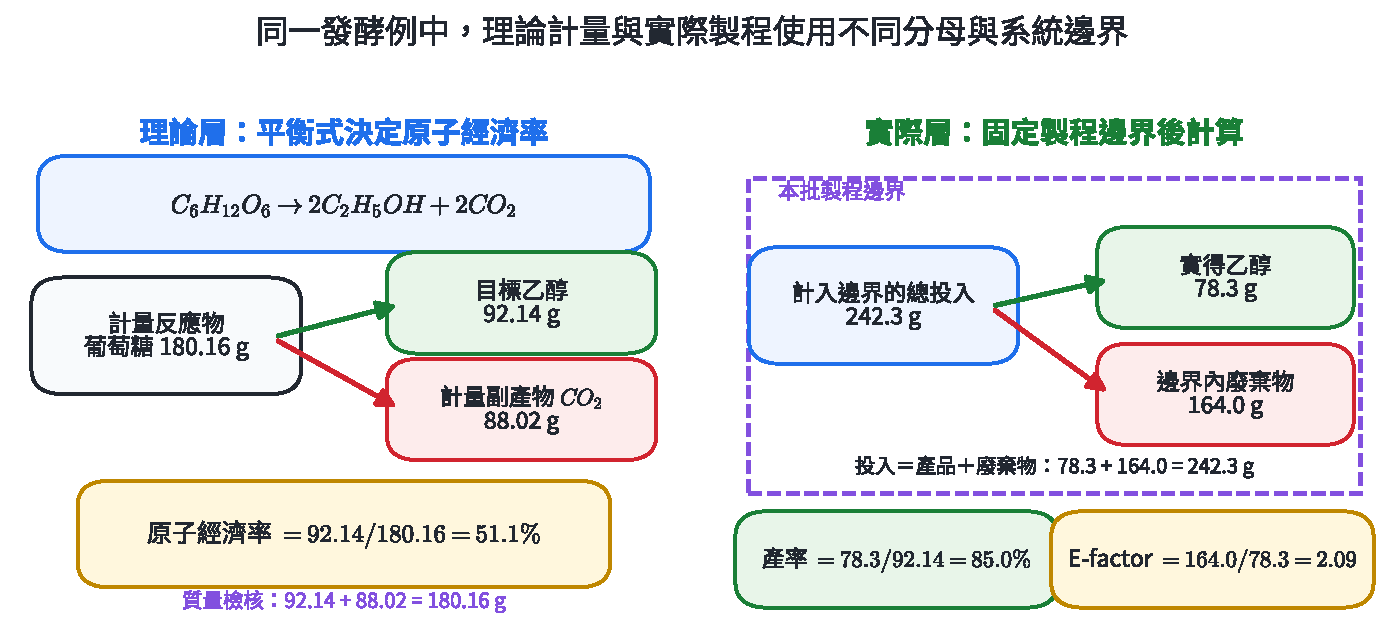
\includegraphics[width=0.98\linewidth,height=\textheight,keepaspectratio,alt={圖 1｜左圖只使用平衡式的理論計量；右圖在另一個實際製程邊界內分配產品與廢棄物。}]{assets/選化V-2-綠色化學物料指標.pdf}
\caption{圖 1｜左圖只使用平衡式的理論計量；右圖在另一個實際製程邊界內分配產品與廢棄物。}
\end{figure}

圖 1 中原子經濟率與產率皆以百分比表示，卻有不同分母；E-factor 沒有百分比單位，且會隨「是否納入水、溶劑與回收物流」的邊界而改變。製程比較至少同時列出物料效率、危害、能耗與產品功能。

\begin{HandoutWorkedExample}

\subsection{示範 1｜由平衡式求發酵的原子經濟率}\label{ux793aux7bc4-1ux7531ux5e73ux8861ux5f0fux6c42ux767cux9175ux7684ux539fux5b50ux7d93ux6fdfux7387}

葡萄糖發酵：

\[
C_6H_{12}O_6\rightarrow2C_2H_5OH+2CO_2.
\]

取 \(M(C_6H_{12}O_6)=180.16\)、\(M(C_2H_5OH)=46.07\ \mathrm{g\ mol^{-1}}\)。目標乙醇的計量質量為 \(2(46.07)=92.14\) g，因此

\[
\text{原子經濟率}=\frac{92.14}{180.16}\times100\%=51.1\%.
\]

其餘計量質量主要成為 \(CO_2\)。此結果由平衡式決定，尚未包含實際發酵不完全、菌體生長或分離用水。

\end{HandoutWorkedExample}

\begin{HandoutWorkedExample}

\subsection{示範 2｜同時比較原子經濟率與產率}\label{ux793aux7bc4-2ux540cux6642ux6bd4ux8f03ux539fux5b50ux7d93ux6fdfux7387ux8207ux7522ux7387}

一條路線每批計量反應物共 \(250\) g，理論目標產物為 \(180\) g，實得 \(153\) g。

\[
\text{原子經濟率}=\frac{180}{250}\times100\%=72.0\%,
\]

\[
\text{產率}=\frac{153}{180}\times100\%=85.0\%.
\]

原子經濟率的損失來自平衡式必然生成的副產物；產率的損失來自實際反應與操作。兩者需分別改善。

\end{HandoutWorkedExample}

\begin{HandoutWorkedExample}

\subsection{示範 3｜固定邊界後比較兩條製程}\label{ux793aux7bc4-3ux56faux5b9aux908aux754cux5f8cux6bd4ux8f03ux5169ux689dux88fdux7a0b}

每生產 \(100\) kg 相同純度產品，路線甲產生 \(210\) kg 廢棄物、使用 \(900\) MJ；路線乙產生 \(130\) kg 廢棄物、使用 \(1250\) MJ。兩者 E-factor 分別為

\[
E_{\text{甲}}=2.10,\qquad E_{\text{乙}}=1.30.
\]

乙在廢棄物指標較佳，甲在能耗較低。若甲使用高毒溶劑、乙使用可回收溶劑，危害結論還會改變。可核對的結論是「乙的物料廢棄物較少、甲的直接能耗較低」，總體選擇需再加入危害、能源來源與回收效率。

\end{HandoutWorkedExample}

\subsection{練習 1}\label{ux7df4ux7fd2-1}

\begin{enumerate}
\def\labelenumi{\arabic{enumi}.}
\tightlist
\item
  加成反應 \(C_2H_4+H_2O\rightarrow C_2H_5OH\) 的原子經濟率為何？
\item
  某反應理論可得 \(50.0\) g 產品，實得 \(41.5\) g；求產率。
\item
  製得 \(80.0\) kg 產品並在既定邊界內產生 \(124\) kg 廢棄物；求 E-factor。
\item
  路線 A 原子經濟率 \(90\%\)、產率 \(60\%\)；路線 B 原子經濟率 \(70\%\)、產率 \(92\%\)。若只知道這兩個數值，可否判定哪條路線的總環境負荷較低？列出還需的兩類資料。
\item
  某反應使用催化劑後，平衡式不變，產率由 \(72\%\) 升至 \(90\%\)，反應溫度由 \(180^\circ\mathrm C\) 降至 \(80^\circ\mathrm C\)。指出原子經濟率、產率與能耗趨勢。
\item
  城市評估以 UV 取代部分含氯消毒。分別列出一項科學、科技、社會與人文層面的必要問題。
\end{enumerate}

\subsection{練習 1 解析}\label{ux7df4ux7fd2-1-ux89e3ux6790}

\begin{enumerate}
\def\labelenumi{\arabic{enumi}.}
\tightlist
\item
  唯一計量產物是乙醇，所有反應物原子都進入目標產物，原子經濟率為 \(100\%\)。
\item
  \(41.5/50.0\times100\%=83.0\%\)。
\item
  \(E=124/80.0=1.55\)，即每 kg 產品對應 \(1.55\) kg 邊界內廢棄物。
\item
  尚不能判定。還需溶劑／助劑與回收物流、能耗及能源來源、原料危害、產品純化與排放毒性等資料；任列兩類並說明邊界即可。
\item
  平衡式不變，所以原子經濟率不變；實得量增加使產率提高；較低溫度通常降低加熱需求，但總能耗仍需納入反應時間、攪拌與分離。
\item
  科學可問 UV 劑量對不同病原的失活曲線與是否留有再生長風險；科技可問燈源、濁度干擾、線上監測與備援；社會可問水價、偏遠地區維護與服務可及性；人文可問風險由誰承受、資訊透明與世代責任。各層問題需用相應證據回答。
\end{enumerate}

綠色化學用於藥物合成、半導體清洗、聚合物設計與水處理製程。物料指標先指出損失發生在哪一層；危害與生命週期資料再決定改善是否把負荷移到其他階段。

\section{2. 科學模型的特性、檢驗與演變}\label{ux79d1ux5b78ux6a21ux578bux7684ux7279ux6027ux6aa2ux9a57ux8207ux6f14ux8b8a}

\subsection{2.1 模型由目的、假設、變數與關係構成}\label{ux6a21ux578bux7531ux76eeux7684ux5047ux8a2dux8b8aux6578ux8207ux95dcux4fc2ux69cbux6210}

\textbf{科學模型}是針對特定目的，保留系統中關鍵物件、變數與關係的表示。模型可以是粒子圖、反應機構、數學方程、電腦模擬或實體裝置。判斷模型品質時需列出：

\begin{itemize}
\tightlist
\item
  目的：要解釋或預測哪個量；
\item
  尺度：空間、時間與濃度範圍；
\item
  假設：哪些因素固定、忽略或平均化；
\item
  可觀測量：能用什麼儀器取得證據；
\item
  預測與不確定度：模型允許哪些結果；
\item
  適用限制：哪些條件改變後需換模型。
\end{itemize}

\begin{figure}
\centering
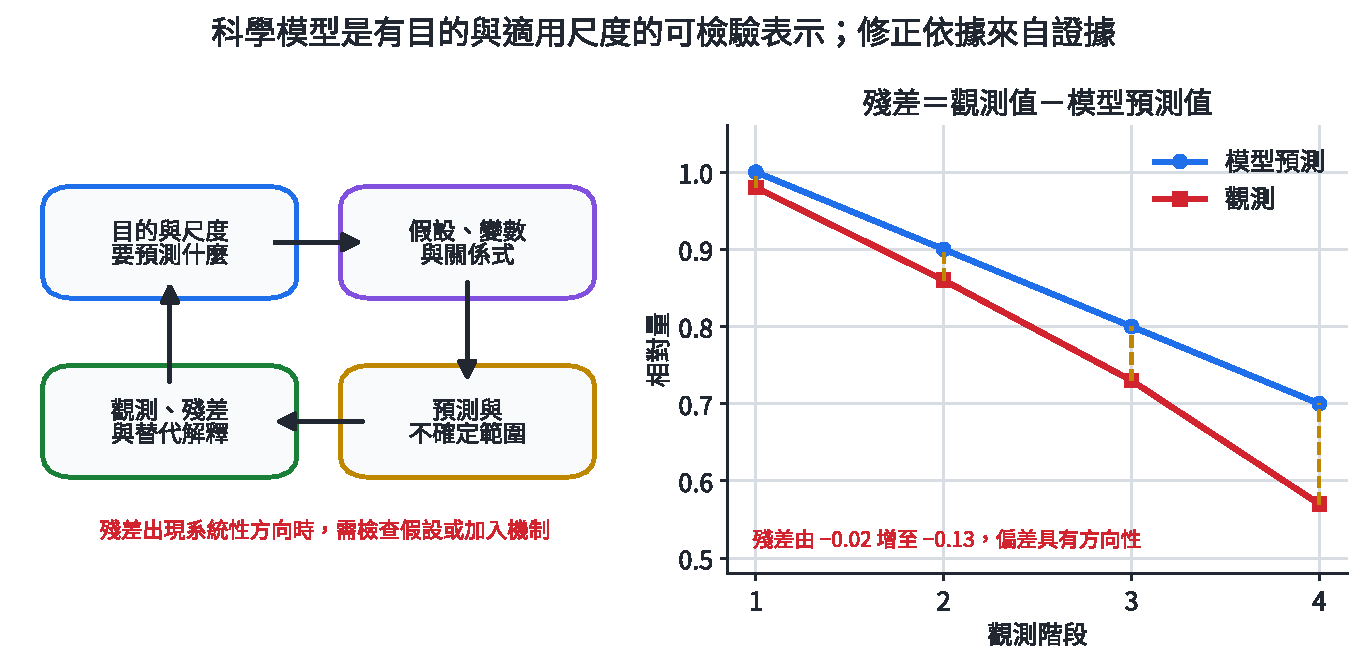
\includegraphics[width=0.98\linewidth,height=\textheight,keepaspectratio,alt={圖 2｜左圖依序連結目的、假設、預測與觀測；右圖用逐步增大的殘差指出模型需要修正。}]{assets/選化V-2-科學模型證據循環.pdf}
\caption{圖 2｜左圖依序連結目的、假設、預測與觀測；右圖用逐步增大的殘差指出模型需要修正。}
\end{figure}

圖 2 右側每條虛線是同一階段的殘差。隨機落在零上下的殘差可來自量測雜訊；持續同方向並逐步增大的殘差表示模型缺少機制、參數隨時間改變，或觀測系統存在校正偏差。

\begin{HandoutWorkedExample}

\subsection{示範 4｜由殘差型態判斷修正方向}\label{ux793aux7bc4-4ux7531ux6b98ux5deeux578bux614bux5224ux65b7ux4feeux6b63ux65b9ux5411}

模型預測某污染物每小時剩餘比例依序為 \(0.90,0.81,0.73,0.66\)；觀測為 \(0.91,0.80,0.69,0.57\)。殘差為

\[
+0.01,-0.01,-0.04,-0.09.
\]

前兩點接近零，後兩點持續為負且幅度增加，表示真實消失速率後期高於模型。可檢驗的修正包含加入光強增加、第二條反應路徑或沉降；先取得光照與生成物資料，再比較替代模型。

\end{HandoutWorkedExample}

\begin{HandoutWorkedExample}

\subsection{示範 5｜分子模型對應的可觀測量與限制}\label{ux793aux7bc4-5ux5206ux5b50ux6a21ux578bux5c0dux61c9ux7684ux53efux89c0ux6e2cux91cfux8207ux9650ux5236}

球棒模型清楚表示鍵結次序與鍵角方向，適合比較順反異構與反應位點；球的半徑、棒的粗細通常不按真實比例，也不直接給出電子密度。若問題是「哪個原子相連」，球棒模型足夠；若問題是「分子表面哪處電子較富集」，需電子密度或靜電勢模型。

\end{HandoutWorkedExample}

\subsection{2.2 臭氧層模型的反應與證據}\label{ux81edux6c27ux5c64ux6a21ux578bux7684ux53cdux61c9ux8207ux8b49ux64da}

平流層中高能紫外光使氧分子光解：

\[
O_2+h\nu\rightarrow2O,
\]

\[
O+O_2+M\rightarrow O_3+M.
\]

\(M\) 是帶走碰撞能量的第三體。臭氧也會光解或與 O 反應，所以臭氧量來自生成與消耗速率的動態平衡。含氯氟烴到達平流層後受紫外光分解，可產生 \(Cl\cdot\)。主要催化循環為

\[
Cl\cdot+O_3\rightarrow ClO\cdot+O_2,
\]

\[
ClO\cdot+O\rightarrow Cl\cdot+O_2.
\]

相加後 \(Cl\cdot\) 與 \(ClO\cdot\) 相消，總反應是 \(O_3+O\rightarrow2O_2\)。自由基再生使少量含氯物質可造成放大效果。

\begin{figure}
\centering
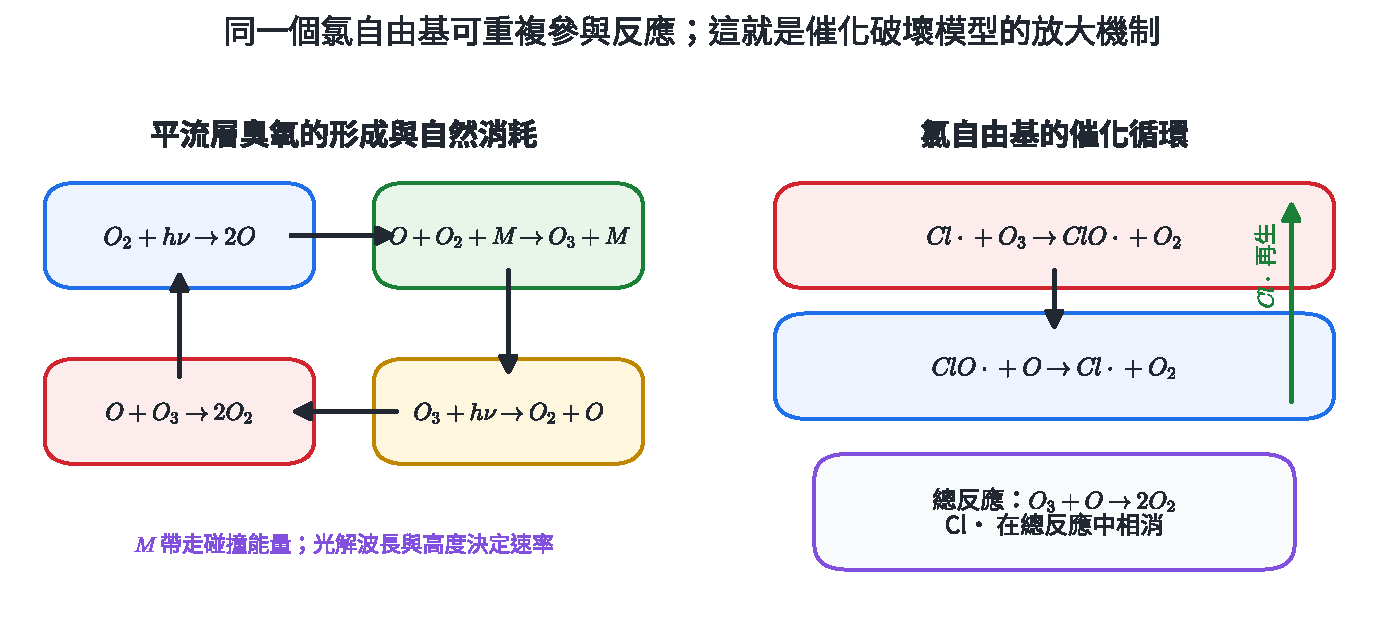
\includegraphics[width=0.98\linewidth,height=\textheight,keepaspectratio,alt={圖 3｜左圖追蹤平流層氧與臭氧的自然循環；右圖把氯自由基相消，得到淨臭氧損失。}]{assets/選化V-2-臭氧生成與氯自由基循環.pdf}
\caption{圖 3｜左圖追蹤平流層氧與臭氧的自然循環；右圖把氯自由基相消，得到淨臭氧損失。}
\end{figure}

圖 3 的模型預測：平流層活性氯增加時，若其餘條件相近，臭氧消耗速率上升；當 \(Cl\cdot\) 被轉成較穩定儲存物種時，催化鏈會暫停。實際大氣還含溴自由基、極區雲表面反應、輸送與季節光照，簡化兩步循環用於建立催化機制，不能單獨重建完整臭氧洞。

\textbf{杜布森單位}（DU）表示單位地表面積上方整個臭氧柱總量。\(1\ \mathrm{DU}=2.69\times10^{16}\) 個 \(O_3\ \mathrm{cm^{-2}}\)；若把臭氧壓到標準狀況，\(1\) DU 對應 \(0.01\) mm 純臭氧厚度。

\begin{figure}
\centering
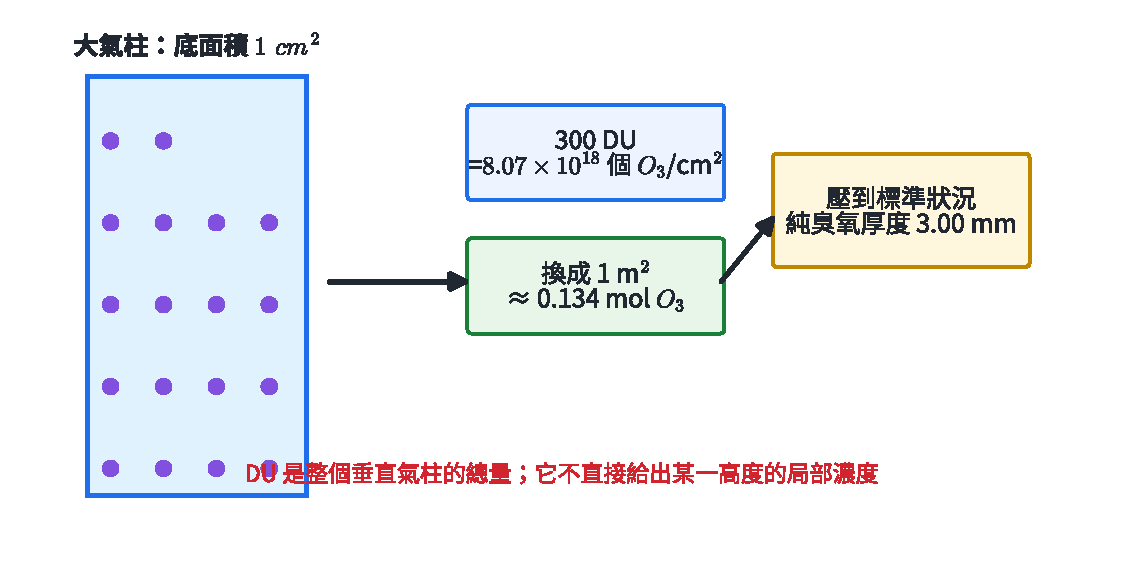
\includegraphics[width=0.96\linewidth,height=\textheight,keepaspectratio,alt={圖 4｜把 300 DU 依序換成每平方公分分子數、每平方公尺莫耳數與標準狀況厚度。}]{assets/選化V-2-臭氧柱量與杜布森單位.pdf}
\caption{圖 4｜把 300 DU 依序換成每平方公分分子數、每平方公尺莫耳數與標準狀況厚度。}
\end{figure}

\begin{HandoutWorkedExample}

\subsection{示範 6｜由反應機構判斷催化劑與總反應}\label{ux793aux7bc4-6ux7531ux53cdux61c9ux6a5fux69cbux5224ux65b7ux50acux5316ux5291ux8207ux7e3dux53cdux61c9}

將圖 3 右側兩式相加：左側有 \(Cl\cdot+ClO\cdot+O_3+O\)，右側有 \(ClO\cdot+Cl\cdot+2O_2\)。約去兩側相同自由基後，得

\[
O_3+O\rightarrow2O_2.
\]

\(Cl\cdot\) 在第一步消耗、第二步再生，未出現在總反應中，是催化物種；\(ClO\cdot\) 是反應中間體。

\end{HandoutWorkedExample}

\begin{HandoutWorkedExample}

\subsection{示範 7｜把臭氧柱量換成不同尺度}\label{ux793aux7bc4-7ux628aux81edux6c27ux67f1ux91cfux63dbux6210ux4e0dux540cux5c3aux5ea6}

\(300\) DU 的純臭氧標準狀況厚度為

\[
300(0.01\ \mathrm{mm})=3.00\ \mathrm{mm}.
\]

每平方公分分子數為

\[
300(2.69\times10^{16})=8.07\times10^{18}\ \mathrm{molecule\ cm^{-2}}.
\]

每平方公尺的莫耳數為

\[
\frac{8.07\times10^{18}\times10^4}{6.022\times10^{23}}
=0.134\ \mathrm{mol\ m^{-2}}.
\]

DU 是垂直整柱總量，尚未指出臭氧集中在哪個高度。

\end{HandoutWorkedExample}

\subsection{練習 2}\label{ux7df4ux7fd2-2}

\begin{enumerate}
\def\labelenumi{\arabic{enumi}.}
\tightlist
\item
  一個箱式模型假設污染物只以一級反應消失。列出至少兩個需固定或量測的條件。
\item
  模型預測值為 \(10.0,8.0,6.4,5.1\)，觀測值為 \(10.1,7.9,6.5,5.0\)。殘差是否呈明顯單向趨勢？
\item
  將 \(O_3+h\nu\rightarrow O_2+O\) 與 \(O+O_3\rightarrow2O_2\) 相加，寫出總反應並指出 O 的角色。
\item
  \(250\) DU 對應標準狀況純臭氧厚度多少 mm？每平方公分有多少個臭氧分子？
\item
  說明平流層臭氧與近地面臭氧在環境作用上的差別，並指出兩者皆為同一化學物種的證據。
\end{enumerate}

\subsection{練習 2 解析}\label{ux7df4ux7fd2-2-ux89e3ux6790}

\begin{enumerate}
\def\labelenumi{\arabic{enumi}.}
\tightlist
\item
  可固定或量測溫度、體積、光照、混合程度、初始濃度、壁面沉降與其他反應物；需至少一項條件支撐速率常數不隨時間改變。
\item
  殘差為 \(+0.1,-0.1,+0.1,-0.1\)，在零上下交替且幅度相近，沒有明顯單向趨勢；它可能在量測不確定度內。
\item
  相加後 O 相消，總反應為 \(2O_3\rightarrow3O_2\)。O 在第一步生成、第二步消耗，是中間體。
\item
  厚度 \(250(0.01)=2.50\) mm；分子數 \(250(2.69\times10^{16})=6.73\times10^{18}\ \mathrm{cm^{-2}}\)。
\item
  平流層臭氧吸收部分紫外光，具有保護作用；近地面高濃度臭氧是刺激性氧化劑，屬二次污染物。兩者分子式皆為 \(O_3\)，差異來自位置、濃度、形成機制與暴露對象。
\end{enumerate}

臭氧模型用於衛星與地面柱量資料的解釋、冷媒管理和紫外線風險評估。模型結論需附時間、空間尺度與不確定度；同一物種在不同高度可有不同環境功能。

\section{3. 水污染、檢測與淨化}\label{ux6c34ux6c61ux67d3ux6aa2ux6e2cux8207ux6de8ux5316}

\subsection{3.1 污染物以來源、形態與作用機制分類}\label{ux6c61ux67d3ux7269ux4ee5ux4f86ux6e90ux5f62ux614bux8207ux4f5cux7528ux6a5fux5236ux5206ux985e}

\textbf{水污染}是物質或能量進入水體，使水質偏離指定用途所需條件。用途不同，合格條件也不同：飲用、灌溉、工業冷卻與維持水生生態會使用不同指標。分析時先指定污染物的化學形態，再追蹤來源、傳輸、轉化與受體。

\begin{itemize}
\tightlist
\item
  \textbf{耗氧有機物}：微生物氧化有機物會消耗溶氧，可能造成低氧。
\item
  \textbf{營養鹽}：含 N、P 物種可促進藻類生長；藻體死亡與分解加重耗氧。
\item
  \textbf{酸、鹼與鹽類}：改變 pH、離子強度與生物可利用性；某些金屬的溶解度也受 pH 控制。
\item
  \textbf{有毒金屬與難分解有機物}：化學形態決定毒性、遷移與是否累積；甲基汞可沿食物鏈放大。
\item
  \textbf{懸浮固體與微塑膠}：造成散射、遮光與棲地覆蓋，也可能攜帶其他污染物。
\item
  \textbf{病原與熱排放}：病原直接影響健康；升溫會改變溶氧飽和度與反應速率。
\end{itemize}

\textbf{溶氧}（DO）是水中溶解 \(O_2\) 的濃度，常以 \(\mathrm{mg\ L^{-1}}\) 表示。DO 受溫度、氣壓、鹽度、混合、光合作用、呼吸與分解共同控制。相同 DO 在不同溫度代表不同飽和度，因此量測時需同時記錄溫度。

\textbf{五日生化需氧量}（\(BOD_5\)）是在規定溫度、暗處、五日培養與適當稀釋條件下，微生物分解樣品中可生物氧化物質所消耗的氧當量。若空白瓶的背景耗氧可忽略，且不需種菌修正，水樣在稀釋瓶中的體積分率為 \(P\)，則

\[
BOD_5=\frac{D_1-D_2}{P},
\]

其中 \(D_1,D_2\) 是培養前後 DO。\textbf{化學需氧量}（COD）以強氧化劑在規定條件下測得氧當量，測定較快，通常涵蓋比 BOD 更多的可氧化物；COD 與 BOD 是方法定義量，不能直接當成某一種化合物的濃度。

\begin{figure}
\centering
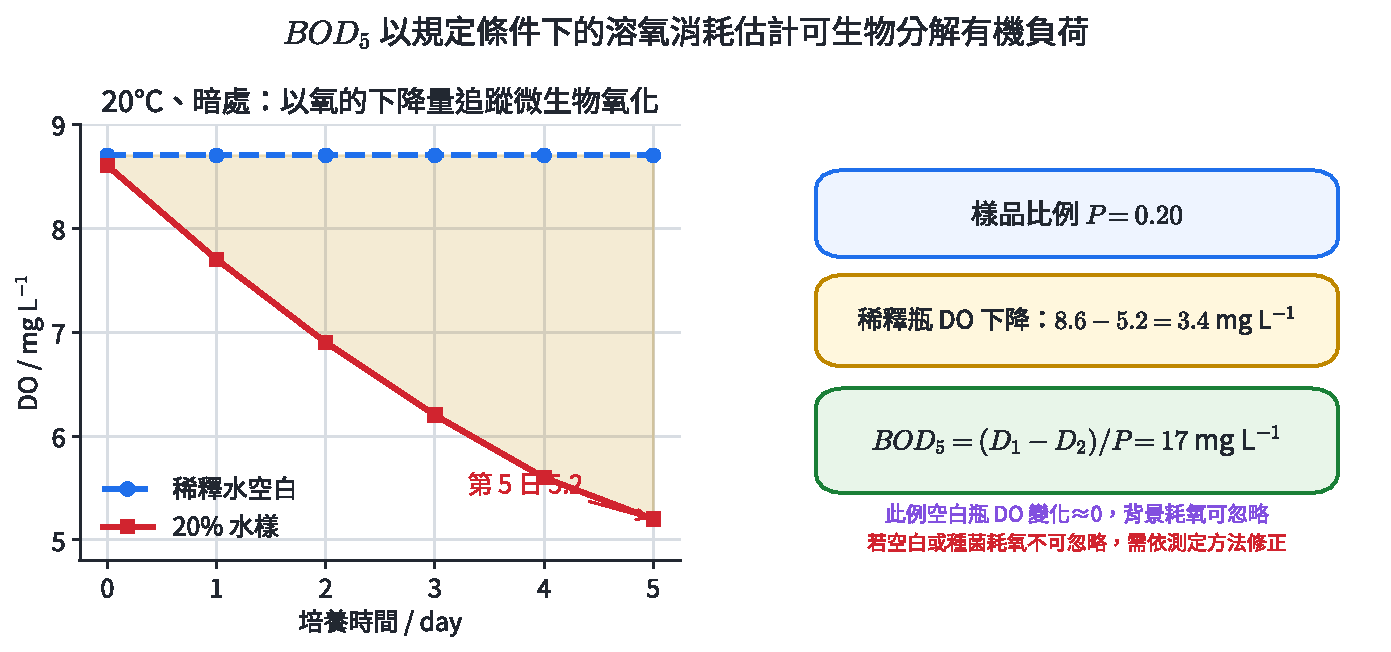
\includegraphics[width=0.98\linewidth,height=\textheight,keepaspectratio,alt={圖 5｜左圖的空白瓶 DO 維持不變，水樣瓶在暗處五日內下降；右圖在此前提下以稀釋比例換算。}]{assets/選化V-2-溶氧與生化需氧量.pdf}
\caption{圖 5｜左圖的空白瓶 DO 維持不變，水樣瓶在暗處五日內下降；右圖在此前提下以稀釋比例換算。}
\end{figure}

\begin{HandoutWorkedExample}

\subsection{\texorpdfstring{示範 8｜由稀釋瓶資料求 \(BOD_5\)}{示範 8｜由稀釋瓶資料求 BOD\_5}}\label{ux793aux7bc4-8ux7531ux7a00ux91cbux74f6ux8cc7ux6599ux6c42-bod_5}

某水樣占稀釋瓶體積的 \(20.0\%\)，初始 DO 為 \(8.6\ \mathrm{mg\ L^{-1}}\)，五日後為 \(5.2\ \mathrm{mg\ L^{-1}}\)；稀釋水空白瓶前後皆為 \(8.7\ \mathrm{mg\ L^{-1}}\)。因此此例的背景耗氧可忽略，

\[
BOD_5=\frac{8.6-5.2}{0.200}=17\ \mathrm{mg\ L^{-1}}.
\]

瓶中直接下降量是 \(3.4\ \mathrm{mg\ L^{-1}}\)；除以 \(P\) 才還原成原水樣的氧當量。暗處可降低藻類光合作用補氧，稀釋可避免 DO 在培養結束前耗盡。

\end{HandoutWorkedExample}

\subsection{3.2 優養化、累積與食物鏈放大}\label{ux512aux990aux5316ux7d2fux7a4dux8207ux98dfux7269ux93c8ux653eux5927}

\textbf{優養化}是水體獲得過多可利用營養鹽，導致生產力上升並改變氧、光與群落結構的過程。因果鏈為：N、P 輸入增加 → 藻類快速增生 → 遮光與藻體死亡 → 分解者耗氧 → 底層低氧或缺氧。白天表層藻類光合作用可暫時提高 DO，夜間呼吸和底層分解則使 DO 降低；單次白天表層 DO 不足以代表整個水體。

\textbf{限制營養鹽}是增加後能明顯提高生物生產量的營養元素。它依水體、季節與化學形態改變，可用平行增肥實驗判斷：對照、加 N、加 P、同時加 N+P，控制水樣體積、光照、溫度與培養時間，再比較葉綠素或藻量。

\begin{figure}
\centering
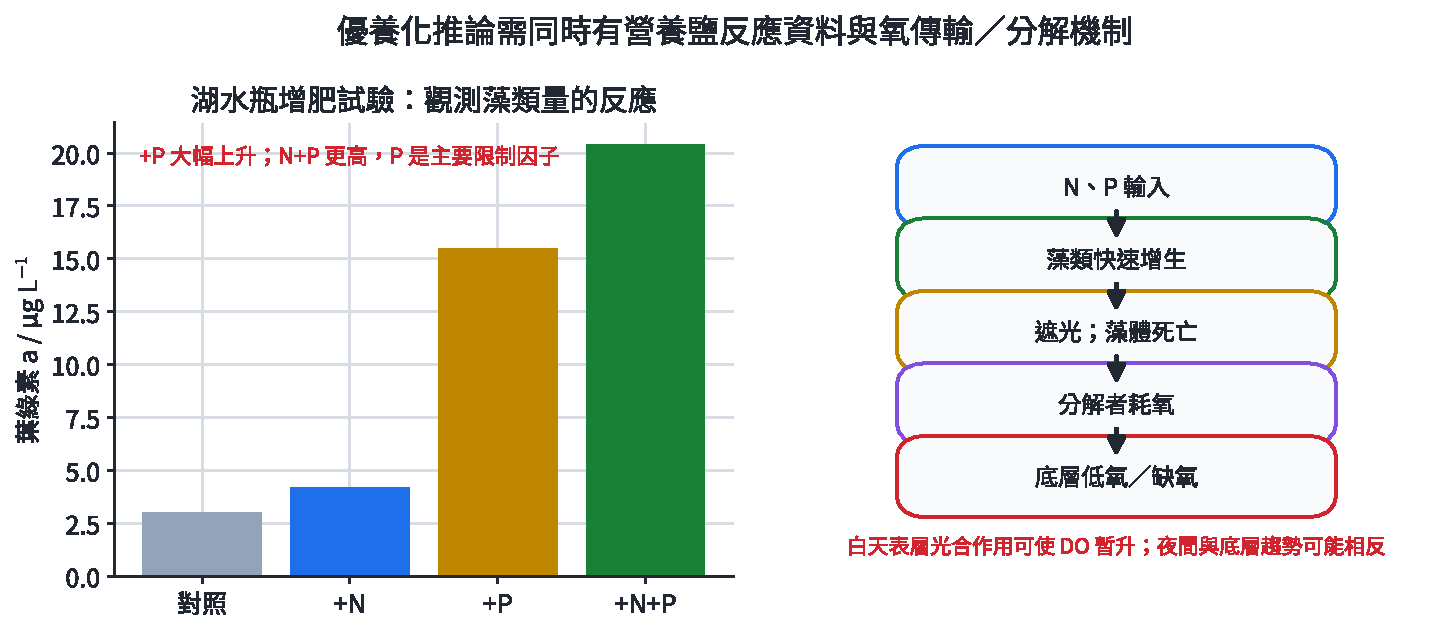
\includegraphics[width=0.98\linewidth,height=\textheight,keepaspectratio,alt={圖 6｜左圖用增肥實驗辨認限制營養鹽；右圖把營養鹽輸入連到缺氧。}]{assets/選化V-2-優養化因果與資料.pdf}
\caption{圖 6｜左圖用增肥實驗辨認限制營養鹽；右圖把營養鹽輸入連到缺氧。}
\end{figure}

\begin{HandoutWorkedExample}

\subsection{示範 9｜由增肥資料判斷限制因子}\label{ux793aux7bc4-9ux7531ux589eux80a5ux8cc7ux6599ux5224ux65b7ux9650ux5236ux56e0ux5b50}

圖 6 中葉綠素 a 依序為：對照 \(3.0\)、加 N \(4.2\)、加 P \(15.5\)、加 N+P \(20.4\ \mu\mathrm{g\,L^{-1}}\)。加 P 的增幅遠大於加 N，表示在此水樣與培養條件下，P 是主要限制因子；N+P 又高於只加 P，表示當 P 限制被解除後，N 或其他交互作用開始影響生長。此結論不自動外推到另一季節或整座湖。

\end{HandoutWorkedExample}

\textbf{生物累積}描述生物體由水、沉積物與食物吸收污染物，而排除或代謝較慢，使體內濃度高於周遭介質。\textbf{生物放大}描述污染物濃度沿營養階層上升。以水中濃度與生物體濃度相除時，質量基準不同，生物濃縮係數（BCF）有 \(\mathrm{L\ kg^{-1}}\) 單位；捕食者與食物都使用 \(\mathrm{mg\ kg^{-1}}\) 時，食物鏈放大係數（BMF）無單位：

\[
BCF=\frac{C_{\text{生物}}\ (\mathrm{mg\ kg^{-1}})}{C_{\text{水}}\ (\mathrm{mg\ L^{-1}})},\qquad
BMF=\frac{C_{\text{捕食者}}\ (\mathrm{mg\ kg^{-1}})}{C_{\text{食物}}\ (\mathrm{mg\ kg^{-1}})}.
\]

\begin{figure}
\centering
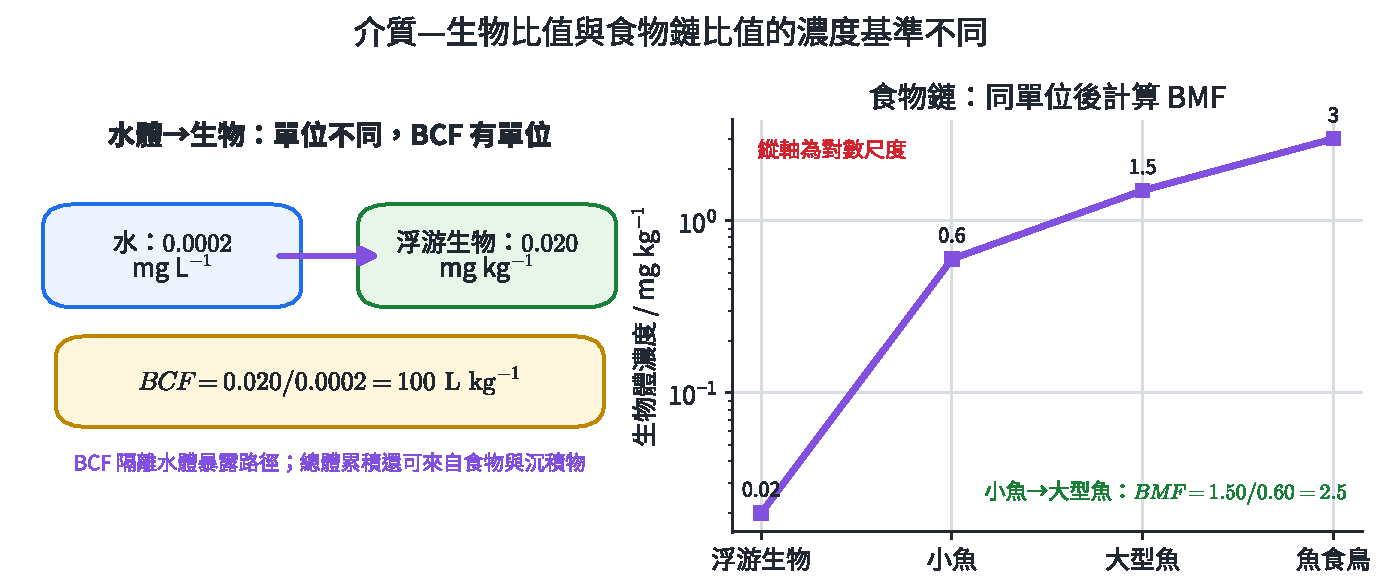
\includegraphics[width=0.98\linewidth,height=\textheight,keepaspectratio,alt={圖 7｜左圖保留水與浮游生物的不同濃度單位；右圖只比較同為 \textbackslash mathrm\{mg\textbackslash{} kg\^{}\{-1\}\} 的食物鏈生物。}]{assets/選化V-2-生物累積與食物鏈放大.pdf}
\caption{圖 7｜左圖保留水與浮游生物的不同濃度單位；右圖只比較同為 \(\mathrm{mg\ kg^{-1}}\) 的食物鏈生物。}
\end{figure}

\begin{HandoutWorkedExample}

\subsection{示範 10｜區分生物濃縮與食物鏈放大}\label{ux793aux7bc4-10ux5340ux5206ux751fux7269ux6fc3ux7e2eux8207ux98dfux7269ux93c8ux653eux5927}

某難分解污染物濃度為：水 \(0.0002\ \mathrm{mg\ L^{-1}}\)、浮游生物 \(0.020\ \mathrm{mg\ kg^{-1}}\)、小魚 \(0.60\ \mathrm{mg\ kg^{-1}}\)、大型魚 \(1.50\ \mathrm{mg\ kg^{-1}}\)。

水到浮游生物的 \(BCF=0.020/0.0002=100\ \mathrm{L\ kg^{-1}}\)；小魚到大型魚的 \(BMF=1.50/0.60=2.5\)。前者比較生物與水，所以保留單位；後者比較同一質量基準的捕食者與食物。組織部位、脂質含量、個體年齡與食性都需一致或校正。

\end{HandoutWorkedExample}

\subsection{練習 3A｜水污染與作用機制}\label{ux7df4ux7fd2-3aux6c34ux6c61ux67d3ux8207ux4f5cux7528ux6a5fux5236}

\begin{enumerate}
\def\labelenumi{\arabic{enumi}.}
\tightlist
\item
  水樣在稀釋瓶中的體積分率為 \(0.25\)，DO 由 \(8.4\) 降至 \(6.1\ \mathrm{mg\ L^{-1}}\)；求 \(BOD_5\)。
\item
  同一湖泊表層中午 DO 高、黎明前 DO 低。以光合作用與呼吸解釋日變化，並說明一次中午量測的限制。
\item
  增肥實驗的葉綠素 a 為：對照 \(2.0\)、加 N \(10.5\)、加 P \(2.6\)、加 N+P \(13.0\ \mu\mathrm{g\,L^{-1}}\)。判斷主要限制營養鹽。
\item
  水中污染物濃度 \(0.001\ \mathrm{mg\ L^{-1}}\)，藻類 \(0.20\ \mathrm{mg\ kg^{-1}}\)，魚 \(1.8\ \mathrm{mg\ kg^{-1}}\)。求水到藻的 BCF 與藻到魚的 BMF。
\item
  甲水樣 \(BOD_5=18\ \mathrm{mg\ L^{-1}}\)、COD \(42\ \mathrm{mg\ L^{-1}}\)；乙水樣分別為 \(4\) 與 \(55\ \mathrm{mg\ L^{-1}}\)。比較兩水樣可生物氧化負荷與全部化學可氧化負荷，並指出 COD－BOD 差值可提供的線索。
\end{enumerate}

\subsection{練習 3A 解析}\label{ux7df4ux7fd2-3a-ux89e3ux6790}

\begin{enumerate}
\def\labelenumi{\arabic{enumi}.}
\tightlist
\item
  \(BOD_5=(8.4-6.1)/0.25=9.2\ \mathrm{mg\ L^{-1}}\)。分子是稀釋瓶的 DO 下降量，分母把結果換回原水樣。
\item
  白天光合作用產氧，中午前後表層 DO 可上升；夜間無光合作用而呼吸持續耗氧，黎明前常較低。一次中午表層值忽略日夜與深度差，不能代表底層最低 DO。
\item
  加 N 使葉綠素由 \(2.0\) 大幅增至 \(10.5\)，加 P 只有小幅變化，故此條件下 N 是主要限制因子；N+P 最高，顯示解除 N 限制後 P 或交互作用仍有影響。
\item
  水到藻：\(BCF=0.20/0.001=200\ \mathrm{L\ kg^{-1}}\)；藻到魚：\(BMF=1.8/0.20=9.0\)。前者的介質與生物濃度基準不同，後者在同一質量基準上相除。
\item
  甲的 \(BOD_5\) 較高，規定五日內的可生物氧化負荷較大；乙的 COD 較高，全部化學可氧化負荷較大。乙的 COD－BOD 差值 \(51\) 大於甲的 \(24\ \mathrm{mg\ L^{-1}}\)，提示乙含較多不易在五日內生物分解、但可被化學氧化的物質；兩個差值仍受方法條件影響。
\end{enumerate}

\subsection{3.3 水質檢測的量、方法與限制}\label{ux6c34ux8ceaux6aa2ux6e2cux7684ux91cfux65b9ux6cd5ux8207ux9650ux5236}

\begin{itemize}
\tightlist
\item
  \textbf{濁度}以粒子對光的散射衡量，校正後常以 NTU 表示。它是光學量，與懸浮固體質量通常相關，卻不等同於特定污染物濃度。
\item
  \textbf{pH}由校正後電極或指示劑測得；電極法需以標準緩衝液校正並控制溫度。
\item
  \textbf{DO}可用電極、滴定或比色法；比色法快速但解析度受色卡、照明與樣品本色影響。
\item
  \textbf{導電度}反映可移動離子的總體導電能力；離子種類與遷移率不同，因此不能只由導電度辨認是哪一種鹽。
\item
  \textbf{BOD、COD、懸浮固體與氨氮}可組成河川污染指標；合成指標需先把不同單位轉成分級或分數。
\end{itemize}

一般濾紙可移除尺寸較大的懸浮固體，對溶解離子、低分子有機物與病原的效果有限。混凝處理加入鋁鹽，使 \(Al^{3+}\) 水解生成絮狀 \(Al(OH)_3\)：

\[
Al^{3+}+3H_2O\rightleftharpoons Al(OH)_3(s)+3H^+.
\]

絮體可吸附或網捕帶電膠體，再經沉澱與過濾移除。明礬有效範圍約在 pH \(4.5\)--\(8.0\)；水解產生 \(H^+\)，水樣鹼度不足時 pH 會下降，影響絮體形成。

\begin{figure}
\centering
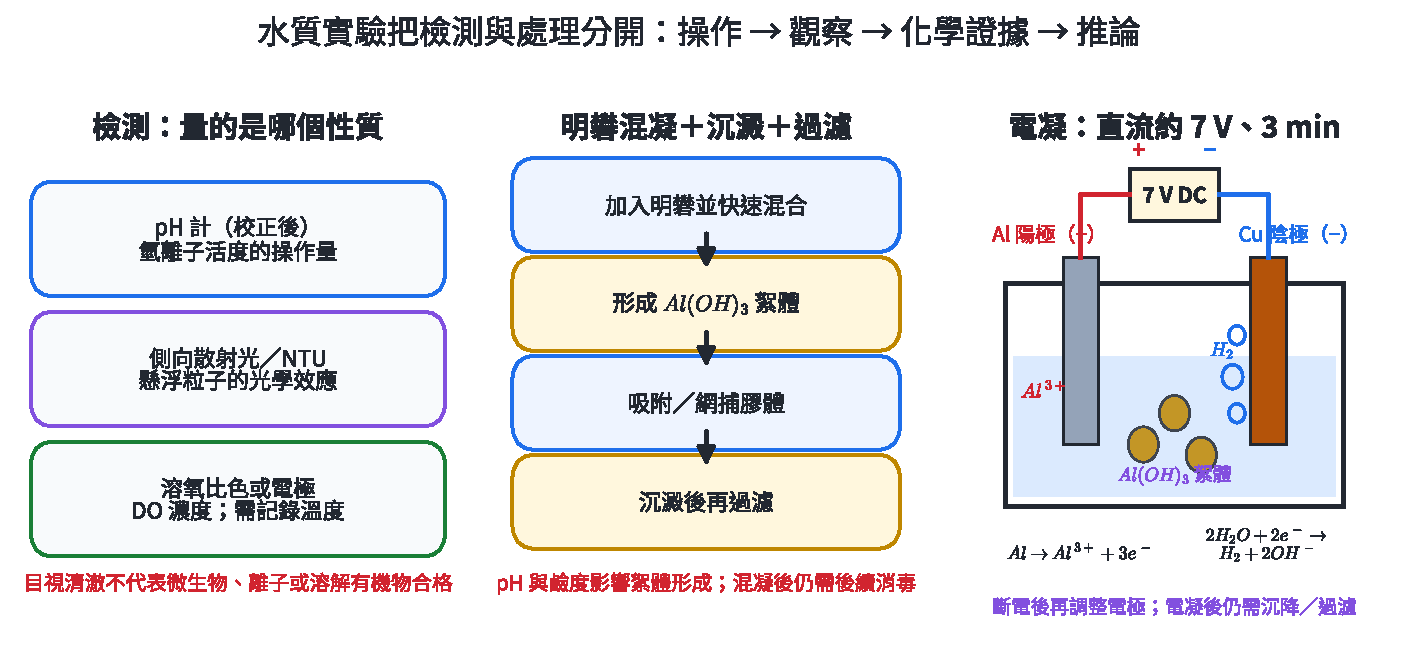
\includegraphics[width=0.99\linewidth,height=\textheight,keepaspectratio,alt={圖 8｜三欄依序建立檢測量、明礬混凝流程，以及直流電源、閉合導線、電極反應與絮體生成的關係。}]{assets/選化V-2-水質檢測與淨化證據鏈.pdf}
\caption{圖 8｜三欄依序建立檢測量、明礬混凝流程，以及直流電源、閉合導線、電極反應與絮體生成的關係。}
\end{figure}

電凝以鋁片作陽極、銅片作陰極，通直流約 \(7\) V。陽極：

\[
Al\rightarrow Al^{3+}+3e^-;
\]

陰極可發生

\[
2H_2O+2e^-\rightarrow H_2+2OH^-.
\]

生成的鋁氫氧化物絮體捕捉膠體，氫氣泡可使部分絮體上浮。電凝後仍需沉降、過濾與依用途進行消毒。

\begin{HandoutWorkedExample}

\subsection{示範 11｜把實驗觀察轉成有限度的推論}\label{ux793aux7bc4-11ux628aux5be6ux9a57ux89c0ux5bdfux8f49ux6210ux6709ux9650ux5ea6ux7684ux63a8ux8ad6}

汙水經濾紙過濾後透光度提高，但雷射光徑仍清楚；加入明礬與碳酸鈉、攪拌靜置再過濾後，雷射光徑明顯變弱。

\begin{enumerate}
\def\labelenumi{\arabic{enumi}.}
\tightlist
\item
  \textbf{觀察}：第一次濾液較清；仍有廷得耳效應。第二次處理後散射減弱。
\item
  \textbf{證據}：大顆粒先被濾紙截留；較小膠體經混凝成較大絮體後才容易過濾。
\item
  \textbf{推論}：混凝改善懸浮／膠體粒子的移除。
\item
  \textbf{限制}：此觀察未檢測溶解鹽、微生物與有毒有機物，不能據此判定可飲用。
\end{enumerate}

\end{HandoutWorkedExample}

\begin{HandoutWorkedExample}

\subsection{示範 12｜由溫度與比色結果求溶氧飽和度}\label{ux793aux7bc4-12ux7531ux6eabux5ea6ux8207ux6bd4ux8272ux7d50ux679cux6c42ux6eb6ux6c27ux98fdux548cux5ea6}

某水樣溫度 \(20^\circ\mathrm C\)，比色結果為 DO \(4\ \mathrm{ppm}\)。題目提供的實驗對照表指出 \(20^\circ\mathrm C\) 時，\(4\) ppm 對應飽和度 \(44\%\)，故直接讀得 \(44\%\)。若另一水樣也是 \(4\) ppm 但溫度為 \(10^\circ\mathrm C\)，需改用 \(10^\circ\mathrm C\) 那一列，因氣體溶解度隨溫度改變。

\end{HandoutWorkedExample}

\subsubsection{水質檢測實驗：安全、操作與證據紀錄}\label{ux6c34ux8ceaux6aa2ux6e2cux5be6ux9a57ux5b89ux5168ux64cdux4f5cux8207ux8b49ux64daux7d00ux9304}

本實驗包含汙水、pH 計、雷射、明礬／碳酸鈉、溶氧測試錠與低電壓直流電凝。

\begin{itemize}
\tightlist
\item
  穿實驗衣、護目鏡與一次性手套；未知水樣視為可能含病原或刺激物，禁止入口與徒手接觸，操作後洗手。
\item
  雷射筆固定朝向黑色背景或水樣，由上向下照射；光束路徑低於眼睛，任何時刻都不指向人眼或反光面。
\item
  電凝使用低電壓直流電源；調整電極前先斷電，雙手與桌面保持乾燥，鋁陽極接正端、銅陰極接負端。
\item
  明礬、碳酸鈉與溶氧測試錠避免吸入、吞食和接觸眼睛；依產品安全資料處理灑漏。
\item
  所有液體樣品、試劑與電凝後液體集中於教師指定廢液桶；濾紙、沉渣與受污染固體進指定固體廢棄桶。未知水樣與含金屬絮體不排入水槽。
\end{itemize}

紀錄表將「操作」「觀察」「推論」分欄。例如「通電 \(3\) min，電流由 \(0.18\) A 降至 \(0.12\) A」是操作與量測；「陽極附近出現白色絮體、陰極有氣泡」是觀察；「鋁溶出並形成氫氧化物，陰極還原水生成氫氣」是以電極反應支持的推論。可用未加混凝劑、未通電但其餘處理相同的水樣作控制組。

\subsection{練習 3B｜水質檢測與淨化}\label{ux7df4ux7fd2-3bux6c34ux8ceaux6aa2ux6e2cux8207ux6de8ux5316}

\begin{enumerate}
\def\labelenumi{\arabic{enumi}.}
\tightlist
\item
  過濾後水樣濁度由 \(36\) NTU 降至 \(8\) NTU，導電度由 \(420\) 降至 \(405\ \mu\mathrm{S\,cm^{-1}}\)。這組資料支持哪些推論？
\item
  電凝時把電源改成交流電會破壞哪個必要條件？寫出鋁陽極半反應，並列一項安全控制。
\item
  pH 計放入 pH \(7.00\) 標準緩衝液時讀得 \(7.28\)。量測水樣前應採取什麼操作？為何不宜只把所有讀值減去 \(0.28\)？
\item
  相同水樣加入明礬 \(0,20,40,80\ \mathrm{mg\ L^{-1}}\) 後，沉澱過濾所得濁度依序為 \(35,11,3,9\) NTU。哪個劑量在此試驗中最佳？說明控制變因與過量時仍需實測的原因。
\item
  實驗紀錄為：「水樣 \(20^\circ\mathrm C\)；比色得 DO \(4\) ppm；依對照表為 \(44\%\) 飽和；水中生物一定因缺氧死亡。」依序標出量測／觀察、資料換算與超出證據的推論，並寫出兩項廢棄物處置。
\end{enumerate}

\subsection{練習 3B 解析}\label{ux7df4ux7fd2-3b-ux89e3ux6790}

\begin{enumerate}
\def\labelenumi{\arabic{enumi}.}
\tightlist
\item
  濁度大幅下降支持大部分散射粒子被移除；導電度只小幅下降，支持多數溶解離子仍在水中。資料未檢測病原與特定毒物。
\item
  電凝需要陽極持續氧化鋁、陰極持續還原水；交流使兩片電極角色反覆交換，難以維持指定反應。陽極為 \(Al\rightarrow Al^{3+}+3e^-\)。安全控制可寫調整電極前斷電、保持手與桌面乾燥或採低電壓直流。
\item
  先依儀器規程以標準緩衝液校正，再沖洗電極並量測。電極偏差可能包含斜率與溫度效應，不必在整個 pH 範圍都等於固定 \(0.28\)，所以不能只作單點常數扣除。
\item
  \(40\ \mathrm{mg\ L^{-1}}\) 得到最低濁度 \(3\) NTU，在這組控制條件下最佳。水樣體積、初始濁度、pH、攪拌、靜置與過濾條件需相同；過量混凝劑可能改變電荷、pH 或留下殘餘物，最佳劑量需用瓶杯試驗而非只假設愈多愈好。
\item
  溫度與比色 DO 是量測／觀察；\(44\%\) 是依指定表格換算；「一定死亡」超出單次 DO 資料，還需物種耐受、持續時間與日夜／深度資料。液體樣品、試劑與電凝液集中進指定廢液桶；濾紙、絮體與受污染固體進指定固體廢棄桶。
\end{enumerate}

水質指標用於汙水處理進出流水監測、河川污染追蹤、養殖溶氧控制與飲用水製程。每個方法只量測特定性質；合格判斷需配合用途、採樣位置、時間、校正與偵測極限。

\section{4. 空氣污染、轉化與空氣品質指標}\label{ux7a7aux6c23ux6c61ux67d3ux8f49ux5316ux8207ux7a7aux6c23ux54c1ux8ceaux6307ux6a19}

\subsection{4.1 一次污染物與二次污染物}\label{ux4e00ux6b21ux6c61ux67d3ux7269ux8207ux4e8cux6b21ux6c61ux67d3ux7269}

\textbf{一次污染物}由來源直接排放，例如不完全燃燒產生的 CO、燃燒高溫形成的 \(NO_x\)、含硫燃料產生的 \(SO_2\)、揮發性有機物（VOC）與一次粒狀物。\textbf{二次污染物}在大氣中由一次污染物經光化學或氧化反應生成，例如近地面 \(O_3\)、硫酸鹽、硝酸鹽與部分二次 \(PM_{2.5}\)。

\begin{figure}
\centering
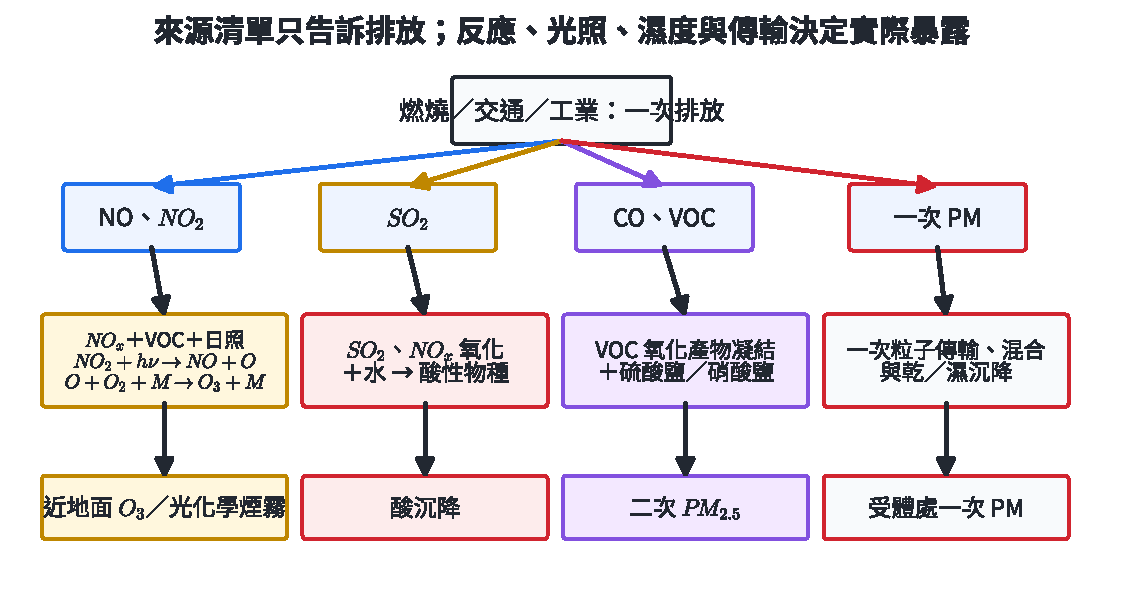
\includegraphics[width=0.99\linewidth,height=\textheight,keepaspectratio,alt={圖 9｜由燃燒與工業排放出發，沿反應箭頭形成近地面臭氧、酸沉降與二次細懸浮微粒。}]{assets/選化V-2-一次與二次空氣污染物.pdf}
\caption{圖 9｜由燃燒與工業排放出發，沿反應箭頭形成近地面臭氧、酸沉降與二次細懸浮微粒。}
\end{figure}

圖 9 顯示「來源」與「受體濃度」之間還有反應與傳輸。風速增加可稀釋本地一次污染物，也可能把污染輸送到下風處；強日照促進光化學反應；濕度與氣膠水相會改變二次粒子生成。監測站濃度是排放、反應、混合與沉降共同結果。

近地面臭氧的簡化生成起始於

\[
NO_2+h\nu\rightarrow NO+O,
\]

\[
O+O_2+M\rightarrow O_3+M.
\]

生成的 \(O_3\) 可與 NO 反應而被消耗；VOC 氧化產生的自由基能把 NO 轉回 \(NO_2\)，卻不必同時消耗 \(O_3\)，因此在日照與前驅物合適時，臭氧可累積。這個機制說明削減方案需考慮 VOC／\(NO_x\) 比、地點與時段。

含硫與含氮污染物氧化後形成酸性物種，可用總體反應表示：

\[
2SO_2+O_2\rightarrow2SO_3,
\]

\[
SO_3+H_2O\rightarrow H_2SO_4,
\]

\[
4NO_2+O_2+2H_2O\rightarrow4HNO_3.
\]

真實大氣可經氣相自由基或雲滴水相路徑；酸沉降包含濕沉降與乾沉降。雨水 pH 只能反映當時淨酸鹼狀態，酸性物質總量還受緩衝鹼、降雨量與解離平衡影響。

\textbf{粒狀污染物}依空氣動力學直徑分類。\(PM_{2.5}\) 表示空氣動力學直徑不大於約 \(2.5\ \mu\mathrm m\) 的粒子群，常用質量濃度 \(\mu\mathrm{g\,m^{-3}}\)。相同質量濃度可能具有不同粒徑分布、表面積與化學組成，因此健康效應還需暴露時間與成分資料。

\begin{HandoutWorkedExample}

\subsection{示範 13｜由反應網路辨認二次污染物}\label{ux793aux7bc4-13ux7531ux53cdux61c9ux7db2ux8defux8fa8ux8a8dux4e8cux6b21ux6c61ux67d3ux7269}

某日早晨交通使 NO 與 VOC 上升；中午日照強，監測到 \(NO_2\) 光解速率增加，下午 \(O_3\) 達高值。NO 與 VOC 是一次排放前驅物，\(O_3\) 是大氣反應生成的二次污染物。臭氧高值晚於交通尖峰，符合「前驅物排放 → 光化學轉化 → 臭氧累積」的時間順序；要確認因果仍需風向、混合層高度與上風處資料。

\end{HandoutWorkedExample}

\begin{HandoutWorkedExample}

\subsection{示範 14｜由 pH 比較氫離子濃度}\label{ux793aux7bc4-14ux7531-ph-ux6bd4ux8f03ux6c2bux96e2ux5b50ux6fc3ux5ea6}

兩場雨的 pH 分別為 \(4.2\) 與 \(5.2\)。依 \([H^+]=10^{-\mathrm{pH}}\)，

\[
\frac{[H^+]_{4.2}}{[H^+]_{5.2}}=10^{-4.2}/10^{-5.2}=10.
\]

pH \(4.2\) 的雨水氫離子濃度是 pH \(5.2\) 的 \(10\) 倍。若要比較總酸沉降量，還需降雨體積、緩衝成分與乾沉降資料。

\end{HandoutWorkedExample}

\subsection{練習 4A｜空氣污染物與大氣轉化}\label{ux7df4ux7fd2-4aux7a7aux6c23ux6c61ux67d3ux7269ux8207ux5927ux6c23ux8f49ux5316}

\begin{enumerate}
\def\labelenumi{\arabic{enumi}.}
\tightlist
\item
  將下列分類為一次或二次污染物：汽機車直接排放的 CO、煙囪排放的 \(SO_2\)、日照下形成的 \(O_3\)、由 \(SO_2\) 氧化形成的硫酸鹽粒子。
\item
  寫出 \(NO_2\) 光解到 \(O_3\) 形成的兩步反應，並說明強日照的作用。
\item
  雨水 pH 由 \(5.6\) 降到 \(4.6\)，\([H^+]\) 增加幾倍？
\item
  甲、乙兩日 PM₂.₅ 質量濃度皆為 \(30\ \mu\mathrm{g\,m^{-3}}\)；甲以粗粒徑無機鹽為主，乙含較多超細燃燒粒子與有機物。這個單一質量濃度能支持什麼結論？還需哪些資料比較健康危害？
\item
  兩天前驅物排放量相近。甲日強日照、弱風、混合層低；乙日多雲、強風、混合層高。預測哪一天本地午後臭氧較易累積，並逐項說明機制。
\end{enumerate}

\subsection{練習 4A 解析}\label{ux7df4ux7fd2-4a-ux89e3ux6790}

\begin{enumerate}
\def\labelenumi{\arabic{enumi}.}
\tightlist
\item
  CO 與 \(SO_2\) 由來源直接排放，屬一次污染物；\(O_3\) 與硫酸鹽粒子在大氣反應後形成，屬二次污染物。
\item
  \(NO_2+h\nu\rightarrow NO+O\)；\(O+O_2+M\rightarrow O_3+M\)。強日照提高能使 \(NO_2\) 光解的光子通量，促進起始步驟。
\item
  \(10^{-4.6}/10^{-5.6}=10\)，增加 \(10\) 倍。
\item
  資料只支持兩日 PM₂.₅ 的質量濃度相同；粒徑數目、表面積與化學組成可能不同。比較健康危害還需粒徑分布、黑碳／金屬／有機物組成、毒理活性、暴露時間與人群資料，任列兩類。
\item
  甲日較易形成並累積本地臭氧：強日照促進 \(NO_2\) 光解；弱風降低稀釋；低混合層把污染限制在較小空氣體積。乙日多雲降低光化學速率，強風與高混合層促進稀釋，但仍需上風處輸送資料確認。
\end{enumerate}

\subsection{4.2 CO 檢測與濃度---暴露尺度}\label{co-ux6aa2ux6e2cux8207ux6fc3ux5ea6ux66b4ux9732ux5c3aux5ea6}

CO 主要來自含碳燃料不完全燃燒。充足氧氣時主要生成 \(CO_2\)；氧氣供應、混合或溫度不足時，CO 比例上升。CO 可與血紅素結合而妨礙氧輸送，因此室內燃燒設備與密閉空間監測特別重要。

電化學 CO 感測器可在工作電極氧化 CO：

\[
CO+H_2O\rightarrow CO_2+2H^++2e^-.
\]

對電極以氧還原維持電荷平衡。經校正後，電流與進入感測器的 CO 通量相關；溫濕度、其他還原性氣體、感測器老化與擴散膜狀態會影響讀值。

\begin{HandoutWorkedExample}

\subsection{示範 15｜由感測器電量估計反應的 CO 量}\label{ux793aux7bc4-15ux7531ux611fux6e2cux5668ux96fbux91cfux4f30ux8a08ux53cdux61c9ux7684-co-ux91cf}

校正實驗中平均電流為 \(1.20\ \mathrm{mA}\)，維持 \(60.0\) s。電量

\[
Q=It=(1.20\times10^{-3})(60.0)=0.0720\ \mathrm C.
\]

電子莫耳數 \(n(e^-)=Q/F=0.0720/96485=7.46\times10^{-7}\) mol。每 mol CO 產生 \(2\) mol 電子，故

\[
n(CO)=\frac{7.46\times10^{-7}}{2}=3.73\times10^{-7}\ \mathrm{mol}.
\]

這是電極反應量；把它換成空氣濃度還需採樣流量、時間、收集效率與校正曲線。

\end{HandoutWorkedExample}

濃度是某時刻、某位置空氣中的物質量比例或質量密度；個人暴露還包含停留時間。若濃度在一段時間近似固定，可用

\[
\text{暴露量指標}\approx C\Delta t
\]

比較同一污染物的暴露。此近似未包含呼吸率、個體敏感性與非線性毒理反應。

\subsection{4.3 AQI 的標準化與最大分指標}\label{aqi-ux7684ux6a19ux6e96ux5316ux8207ux6700ux5927ux5206ux6307ux6a19}

空氣品質指標先把不同污染物濃度依各自斷點轉為無因次分指標，再取最大值作當時 AQI。若濃度 \(C\) 位於斷點 \(C_{lo},C_{hi}\)，對應分指標 \(I_{lo},I_{hi}\)，線性內插為

\[
I=\frac{I_{hi}-I_{lo}}{C_{hi}-C_{lo}}(C-C_{lo})+I_{lo}.
\]

法規斷點與平均時間可能更新，解題以題目提供的表為準；實務判讀使用當時主管機關公告。

\begin{figure}
\centering
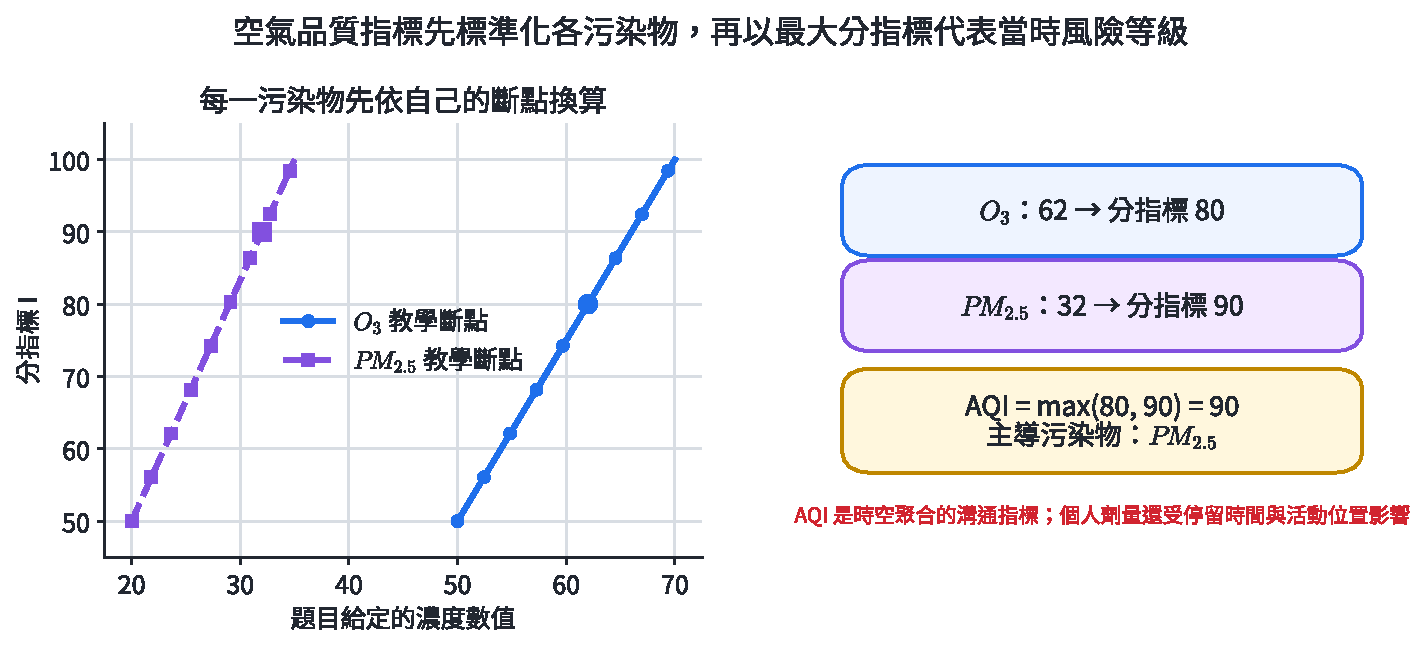
\includegraphics[width=0.98\linewidth,height=\textheight,keepaspectratio,alt={圖 10｜左圖對兩種污染物各自線性內插；右圖顯示 AQI 取較大的 PM2.5 分指標。}]{assets/選化V-2-AQI分指標與最大值.pdf}
\caption{圖 10｜左圖對兩種污染物各自線性內插；右圖顯示 AQI 取較大的 PM2.5 分指標。}
\end{figure}

\begin{HandoutWorkedExample}

\subsection{示範 16｜由題目斷點計算 AQI}\label{ux793aux7bc4-16ux7531ux984cux76eeux65b7ux9edeux8a08ux7b97-aqi}

題目給 O₃：\(50\to I=50\)、\(70\to I=100\)，測得 \(62\)；PM₂.₅：\(20\to I=50\)、\(35\to I=100\)，測得 \(32\)。

\[
I_{O_3}=\frac{50}{20}(62-50)+50=80,
\]

\[
I_{PM}=\frac{50}{15}(32-20)+50=90.
\]

因此 \(AQI=\max(80,90)=90\)，主導污染物為 PM₂.₅。兩個原始濃度單位不同，先轉成分指標後才可比較。

\end{HandoutWorkedExample}

\textbf{危害}是物質造成傷害的固有能力；\textbf{暴露}描述劑量、途徑與時間；\textbf{風險}由危害與暴露共同決定。AQI 是區域與時間平均後的溝通指標，不能完全代表個人在室內、通勤或運動時的實際吸入劑量。

\subsection{練習 4B｜空氣檢測、AQI 與暴露}\label{ux7df4ux7fd2-4bux7a7aux6c23ux6aa2ux6e2caqi-ux8207ux66b4ux9732}

\begin{enumerate}
\def\labelenumi{\arabic{enumi}.}
\tightlist
\item
  CO 感測器在 \(2.00\ \mathrm{mA}\) 下工作 \(120\) s；依每 mol CO 轉移 \(2\) mol 電子，求反應的 CO 莫耳數，取 \(F=9.65\times10^4\ \mathrm{C\ mol^{-1}}\)。
\item
  題目給污染物 X 的斷點 \(C=40\to I=50\)、\(C=60\to I=100\)，測得 \(C=54\)；污染物 Y 的分指標為 \(72\)。求 X 分指標、AQI 與主導污染物。
\item
  兩人都處在 \(35\ \mu\mathrm{g\,m^{-3}}\) 的 PM₂.₅；甲停留 \(1.0\) h，乙停留 \(4.0\) h。以 \(C\Delta t\) 比較暴露指標，並列一項此比較未包含的因素。
\item
  題目給 O₃ 分指標 \(88\)、PM₂.₅ 分指標 \(105\)、CO 分指標 \(43\)。求 AQI、主導污染物，並說明為何不能取三者平均。
\item
  CO 感測器在零 CO、含乙醇蒸氣時也出現訊號。設計一組最少三個氣體條件的校正／干擾實驗，並指出讀值要換成 CO 濃度還需的流量資料。
\end{enumerate}

\subsection{練習 4B 解析}\label{ux7df4ux7fd2-4b-ux89e3ux6790}

\begin{enumerate}
\def\labelenumi{\arabic{enumi}.}
\tightlist
\item
  \(Q=It=(2.00\times10^{-3})(120)=0.240\ \mathrm C\)；\(n(e^-)=0.240/(9.65\times10^4)=2.49\times10^{-6}\) mol；\(n(CO)=1.24\times10^{-6}\) mol。
\item
  \(I_X=50+(54-40)(50/20)=85\)。AQI 取 \(\max(85,72)=85\)，主導污染物為 X。
\item
  甲為 \(35\ \mu\mathrm{g\,h\,m^{-3}}\)，乙為 \(140\ \mu\mathrm{g\,h\,m^{-3}}\)，乙是甲的 \(4\) 倍。未包含呼吸率、口罩、室內外滲透、粒子成分或個體敏感性，任列一項即可。
\item
  \(AQI=\max(88,105,43)=105\)，主導污染物為 PM₂.₅。AQI 的定義是最大分指標，用來保留當下最不利污染物；平均會把高值稀釋。
\item
  至少包含零氣體、已知 CO、已知乙醇三組；若資源允許再加 CO＋乙醇混合物以檢查加成性。控制溫濕度、流量與時間，建立 CO 靈敏度及乙醇交叉靈敏度。換算空氣濃度還需採樣流量／通過體積與感測器收集效率。
\end{enumerate}

空氣污染模型用於排放控制、監測站選址、健康警示與跨區傳輸分析。濃度高值需同時檢查前驅物、光照、氣象與量測時間；氣候作用則常以多年、全球尺度分析，時間尺度與健康 AQI 不同。

\section{5. 化學與永續發展}\label{ux5316ux5b78ux8207ux6c38ux7e8cux767cux5c55}

\subsection{5.1 永續比較先固定功能、邊界與尺度}\label{ux6c38ux7e8cux6bd4ux8f03ux5148ux56faux5b9aux529fux80fdux908aux754cux8207ux5c3aux5ea6}

\textbf{永續發展}是在滿足當代需求時，保留未來世代滿足其需求的能力。化學分析可量化原料、能源、排放與危害；完整判斷還包含資源可及性、健康、公平與技術韌性。可比較的評估需先寫出三項：

\begin{enumerate}
\def\labelenumi{\arabic{enumi}.}
\tightlist
\item
  \textbf{功能單位}：被比較系統提供的相同服務，例如「交付 \(1\) MJ 可用能」或「處理 \(1\ \mathrm{m^3}\) 原水至同一水質」。
\item
  \textbf{系統邊界}：是否包含原料取得、製造、運輸、使用、維修、回收與最終處置。
\item
  \textbf{時間與空間尺度}：一批、一年或整個壽命；工廠、流域或全球。
\end{enumerate}

物料平衡是環境分析的基礎。對指定控制體與時間範圍：

\[
\text{輸入}-\text{輸出}+\text{生成}-\text{消耗}=\text{累積}.
\]

若追蹤元素總量，化學反應不生成或消耗元素，生成與消耗項可合併到物種轉化；若追蹤某一化合物，反應生成與消耗就必須列出。

\begin{HandoutWorkedExample}

\subsection{示範 17｜由控制體求未知排放}\label{ux793aux7bc4-17ux7531ux63a7ux5236ux9ad4ux6c42ux672aux77e5ux6392ux653e}

某處理廠一天進入 \(500\) kg 有機碳；回收產品含 \(280\) kg C，生物污泥含 \(90\) kg C，池內累積 \(20\) kg C，氣相與出流水的碳合計未知。元素碳守恆：

\[
500=280+90+20+x,
\]

故 \(x=110\) kg C day\(^{-1}\)。此差額只給出「氣相＋出流水」總碳，若要分辨 \(CO_2\)、\(CH_4\) 與溶解有機碳，需各自量測或建立物種模型。

\end{HandoutWorkedExample}

\begin{HandoutWorkedExample}

\subsection{示範 18｜同一物質的危害與暴露情境}\label{ux793aux7bc4-18ux540cux4e00ux7269ux8ceaux7684ux5371ux5bb3ux8207ux66b4ux9732ux60c5ux5883}

清潔劑 A 具有較高皮膚刺激性，但在密閉自動設備中每班使用 \(0.10\) kg；清潔劑 B 刺激性較低，卻由人工開放噴灑每班 \(8.0\) kg。危害資料支持 A 的固有刺激性較高；暴露資料可能使 B 的吸入與皮膚接觸較大。風險比較需加入揮發性、濃度、通風、防護具與接觸時間，不能只依「毒性高低」或「使用量」單軸判定。

\end{HandoutWorkedExample}

\subsection{5.2 濃度、總量與通量}\label{ux6fc3ux5ea6ux7e3dux91cfux8207ux901aux91cf}

\textbf{濃度}描述單位體積或質量中的含量；\textbf{總量}等於濃度乘上相應體積或質量；\textbf{通量}描述單位時間穿過邊界的量。河流污染負荷常用

\[
L=CQ,
\]

其中 \(C\) 是質量濃度，\(Q\) 是流量，\(L\) 是質量／時間。兩條河濃度相同，流量較大的河每小時輸送總量較大；只比較濃度不能回答下游每日承受的總負荷。

\begin{HandoutWorkedExample}

\subsection{示範 19｜由濃度與流量求污染負荷}\label{ux793aux7bc4-19ux7531ux6fc3ux5ea6ux8207ux6d41ux91cfux6c42ux6c61ux67d3ux8ca0ux8377}

出流水硝酸根氮濃度為 \(12\ \mathrm{mg\ N\ L^{-1}}\)，流量為 \(2.5\times10^6\ \mathrm{L\ day^{-1}}\)：

\[
L=(12)(2.5\times10^6)=3.0\times10^7\ \mathrm{mg\ N\ day^{-1}}
=30\ \mathrm{kg\ N\ day^{-1}}.
\]

若濃度降為一半但流量加倍，負荷仍為 \(30\ \mathrm{kg\ day^{-1}}\)。

\end{HandoutWorkedExample}

\subsection{練習 5}\label{ux7df4ux7fd2-5}

\begin{enumerate}
\def\labelenumi{\arabic{enumi}.}
\tightlist
\item
  比較紙杯與可重複使用杯時，寫出一個合理功能單位與至少三個生命週期階段。
\item
  某湖一天流入總磷 \(48\) kg，流出 \(31\) kg，沉積固定 \(12\) kg；忽略其他反應，求湖中累積量。
\item
  廢水濃度 \(5.0\ \mathrm{mg\ L^{-1}}\)、流量 \(8.0\times10^5\ \mathrm{L\ day^{-1}}\)；求每日負荷 kg day\(^{-1}\)。
\item
  兩製程都生產 \(1\) kg 相同純度產品。甲直接排放低但使用大量一次性溶劑；乙直接能耗高但溶劑回收率 \(95\%\)。指出比較前需一致的邊界與至少一個性能資料。
\item
  「天然來源」是否足以推出低風險？以危害與暴露各寫一項需量測資料。
\end{enumerate}

\subsection{練習 5 解析}\label{ux7df4ux7fd2-5-ux89e3ux6790}

\begin{enumerate}
\def\labelenumi{\arabic{enumi}.}
\tightlist
\item
  功能單位可定為「完成 \(1000\) 次、每次 \(300\) mL 飲用服務」。階段可列原料取得、杯體製造、運輸、清洗／使用、回收或處置；至少三項且兩種杯採相同邊界。
\item
  累積 \(=48-31-12=5\) kg day\(^{-1}\)。
\item
  \(L=(5.0)(8.0\times10^5)=4.0\times10^6\) mg day\(^{-1}=4.0\) kg day\(^{-1}\)。
\item
  邊界需一致納入溶劑製造、回收所需能耗與溶劑損失、產品分離和廢棄物處置。性能資料可用產率、純度、處理量、設備壽命或安全控制效果。
\item
  不足。危害需量測急慢性毒性、腐蝕性或致敏性；暴露需量測濃度、用量、揮發性、接觸途徑與時間，任各列一項即可。
\end{enumerate}

功能單位與系統邊界使製程、材料與政策的比較可重算。結論需保留取捨：一項指標改善時，能耗、稀缺材料、毒性或風險可能移到別的生命週期階段。

\section{6. 氮循環與農業氮收支}\label{ux6c2eux5faaux74b0ux8207ux8fb2ux696dux6c2eux6536ux652f}

\subsection{6.1 氮的主要物種與微生物轉化}\label{ux6c2eux7684ux4e3bux8981ux7269ux7a2eux8207ux5faeux751fux7269ux8f49ux5316}

大氣 \(N_2\) 的 N 為 \(0\)；\(NH_3/NH_4^+\) 中為 \(-3\)；\(NO_2^-\) 中為 \(+3\)；\(NO_3^-\) 中為 \(+5\)。氮循環的主要過程為：

\begin{itemize}
\tightlist
\item
  \textbf{固氮}：\(N_2\) 轉成可被生物利用的還原態氮；可由固氮微生物、閃電或工業哈柏法完成。
\item
  \textbf{同化}：生物吸收 \(NH_4^+\) 或 \(NO_3^-\)，合成胺基酸、核酸等有機氮。
\item
  \textbf{氨化}：分解者把有機氮轉成 \(NH_3/NH_4^+\)。
\item
  \textbf{硝化}：需氧微生物依序把 \(NH_4^+\) 氧化為 \(NO_2^-\)、\(NO_3^-\)。
\item
  \textbf{反硝化}：缺氧條件下以 \(NO_3^-\) 作電子受體，還原成 \(N_2\) 或中間含氮氣體。
\end{itemize}

\begin{figure}
\centering
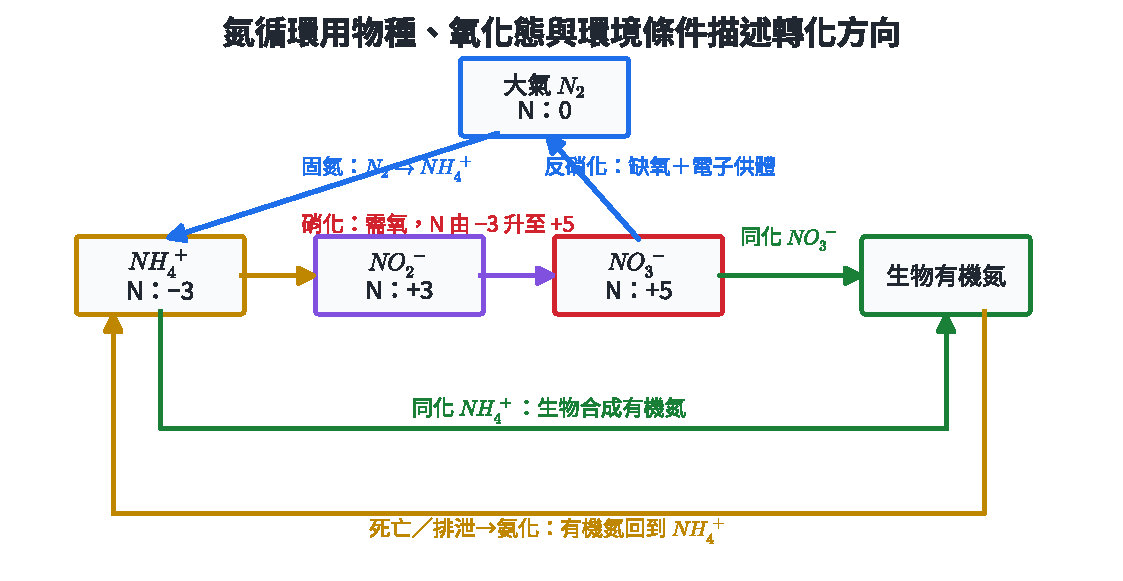
\includegraphics[width=0.98\linewidth,height=\textheight,keepaspectratio,alt={圖 11｜每個氮庫標出化學物種與 N 氧化數；NH\_4\^{}+ 與 NO\_3\^{}- 各有獨立同化箭頭，有機氮再經氨化回到 NH\_4\^{}+。}]{assets/選化V-2-氮循環物種與氧化態.pdf}
\caption{圖 11｜每個氮庫標出化學物種與 N 氧化數；\(NH_4^+\) 與 \(NO_3^-\) 各有獨立同化箭頭，有機氮再經氨化回到 \(NH_4^+\)。}
\end{figure}

硝化的總體氧化可近似寫成

\[
NH_4^++2O_2\rightarrow NO_3^-+2H^++H_2O.
\]

因此硝化消耗氧並產生酸度；曝氣不足時速率會下降。反硝化需缺氧環境與電子供體，能移除水中硝酸鹽，但也可能生成 \(N_2O\) 等中間產物；氧、碳源與停留時間會改變產物分布。

\begin{HandoutWorkedExample}

\subsection{示範 20｜用氧化數判斷硝化方向}\label{ux793aux7bc4-20ux7528ux6c27ux5316ux6578ux5224ux65b7ux785dux5316ux65b9ux5411}

\(NH_4^+\) 中 N 為 \(-3\)，\(NO_3^-\) 中 N 為 \(+5\)，每 mol N 的氧化數上升 \(8\)，表示氮失去 \(8\) mol 電子當量而被氧化。\(O_2\) 作電子受體並被還原成水。由總反應可見每 mol \(NH_4^+\) 消耗 \(2\) mol \(O_2\)，並生成 \(2\) mol \(H^+\)。

\end{HandoutWorkedExample}

\begin{HandoutWorkedExample}

\subsection{示範 21｜判斷處理槽條件對氮物種的影響}\label{ux793aux7bc4-21ux5224ux65b7ux8655ux7406ux69fdux689dux4ef6ux5c0dux6c2eux7269ux7a2eux7684ux5f71ux97ff}

第一槽充分曝氣，第二槽停止曝氣並加入可生物分解碳源。第一槽提供硝化所需 \(O_2\)，預期 \(NH_4^+\) 降低、\(NO_3^-\) 增加；第二槽缺氧且有電子供體，促進反硝化，預期 \(NO_3^-\) 降低、\(N_2\) 生成。若第二槽仍有高 DO，反硝化微生物會優先使用氧，硝酸鹽去除效果下降。

\end{HandoutWorkedExample}

\subsection{6.2 肥料、哈柏法與環境負荷}\label{ux80a5ux6599ux54c8ux67cfux6cd5ux8207ux74b0ux5883ux8ca0ux8377}

哈柏法以

\[
N_2+3H_2\rightleftharpoons2NH_3
\]

將大氣氮轉成氨，支撐肥料與含氮化學品。反應本身的原子經濟率為 \(100\%\)；實際環境負荷主要來自製氫、壓縮加熱、未轉化氣體循環與肥料使用後的流失。若 \(H_2\) 由化石燃料製得，伴隨的 \(CO_2\) 需納入生命週期；以低碳電力電解水製氫時，電力需求與設備材料成為重要項目。

農田施入的氮可進入作物、土壤有機質、氨揮發、反硝化氣體、淋洗或逕流。對指定田區與一季建立收支：

\[
N_{\text{輸入}}=N_{\text{收穫}}+N_{\text{氣體}}+N_{\text{水輸出}}+N_{\text{土壤累積}}.
\]

\begin{figure}
\centering
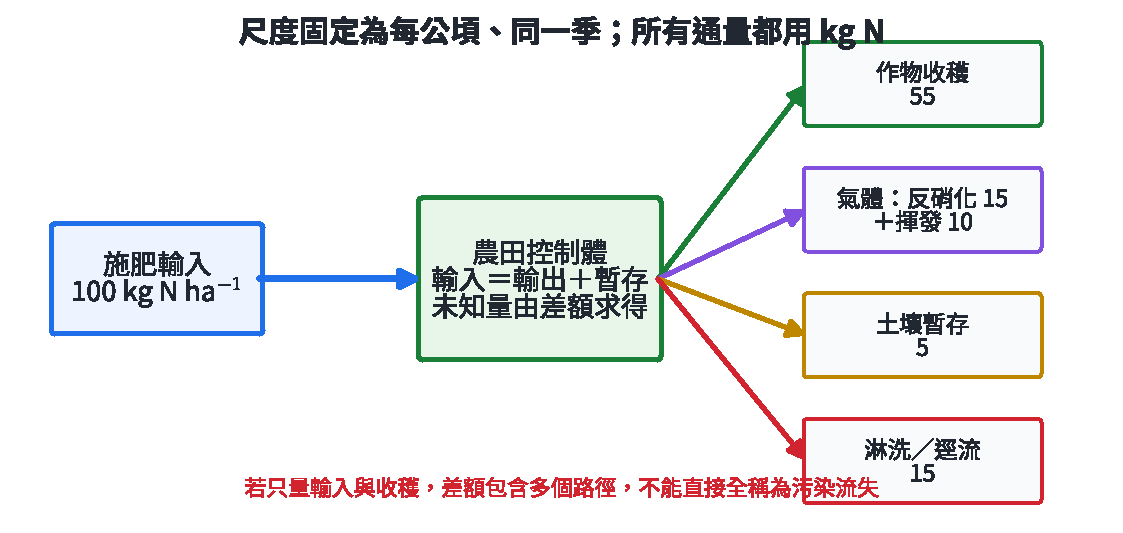
\includegraphics[width=0.98\linewidth,height=\textheight,keepaspectratio,alt={圖 12｜以每公頃、同一季為控制體，把 100 kg N 輸入分配到作物、氣體、土壤與水輸出。}]{assets/選化V-2-農田氮收支.pdf}
\caption{圖 12｜以每公頃、同一季為控制體，把 100 kg N 輸入分配到作物、氣體、土壤與水輸出。}
\end{figure}

\begin{HandoutWorkedExample}

\subsection{示範 22｜由農田氮帳本求淋洗與逕流}\label{ux793aux7bc4-22ux7531ux8fb2ux7530ux6c2eux5e33ux672cux6c42ux6dcbux6d17ux8207ux9015ux6d41}

每公頃施肥 \(100\) kg N；作物收穫帶走 \(55\) kg，反硝化 \(15\) kg，氨揮發 \(10\) kg，土壤暫存 \(5\) kg。由守恆：

\[
N_{\text{水輸出}}=100-55-15-10-5=15\ \mathrm{kg\ N\ ha^{-1}}.
\]

這是淋洗與逕流合計；若要連到河川濃度，還需水量、路徑與時間分布。

\end{HandoutWorkedExample}

\begin{HandoutWorkedExample}

\subsection{示範 23｜由濃度與排水量求硝酸鹽氮流失}\label{ux793aux7bc4-23ux7531ux6fc3ux5ea6ux8207ux6392ux6c34ux91cfux6c42ux785dux9178ux9e7dux6c2eux6d41ux5931}

田區排水量為 \(1.2\times10^6\ \mathrm{L}\)，平均硝酸鹽氮濃度 \(8.0\ \mathrm{mg\ N\ L^{-1}}\)：

\[
m=(8.0)(1.2\times10^6)=9.6\times10^6\ \mathrm{mg\ N}=9.6\ \mathrm{kg\ N}.
\]

若收支差額為 \(15\) kg N，尚有 \(5.4\) kg 可能經其他水路、未採樣時段或量測不確定度；差額提示需補量測，不直接指定唯一去向。

\end{HandoutWorkedExample}

\subsection{練習 6}\label{ux7df4ux7fd2-6}

\begin{enumerate}
\def\labelenumi{\arabic{enumi}.}
\tightlist
\item
  求 \(NH_4^+\)、\(NO_2^-\)、\(NO_3^-\) 中 N 的氧化數，排列 N 的氧化程度。
\item
  依 \(NH_4^++2O_2\rightarrow NO_3^-+2H^++H_2O\)，\(0.50\) mol \(NH_4^+\) 完全硝化消耗多少 mol \(O_2\)、生成多少 mol \(H^+\)？
\item
  說明汙水處理為何常把好氧硝化槽與缺氧反硝化槽分開。
\item
  一季輸入 \(120\) kg N；收穫 \(66\) kg、氣體損失 \(24\) kg、土壤累積 \(12\) kg。求水輸出。
\item
  河川流量 \(4.0\times10^7\ \mathrm{L\ day^{-1}}\)，硝酸鹽氮 \(3.5\ \mathrm{mg\ L^{-1}}\)；求每日氮負荷 kg day\(^{-1}\)，並說明高負荷與優養化的連結。
\end{enumerate}

\subsection{練習 6 解析}\label{ux7df4ux7fd2-6-ux89e3ux6790}

\begin{enumerate}
\def\labelenumi{\arabic{enumi}.}
\tightlist
\item
  依 H 為 \(+1\)、O 為 \(-2\)：\(NH_4^+\) 中 N 為 \(-3\)，\(NO_2^-\) 為 \(+3\)，\(NO_3^-\) 為 \(+5\)；氧化程度依序上升。
\item
  係數比 \(NH_4^+:O_2:H^+=1:2:2\)，故消耗 \(1.0\) mol \(O_2\)，生成 \(1.0\) mol \(H^+\)。
\item
  硝化菌需要氧把還原態氮氧化；反硝化需要缺氧條件，使微生物以硝酸根作電子受體。分槽可分別控制 DO、碳源與停留時間。
\item
  水輸出 \(=120-66-24-12=18\) kg N。
\item
  \(L=(3.5)(4.0\times10^7)=1.4\times10^8\) mg day\(^{-1}=140\) kg day\(^{-1}\)。可利用氮輸入水體後促進藻類生長，藻體死亡分解會耗氧；實際限制因子仍需 N／P 與生物反應資料。
\end{enumerate}

氮循環模型用於肥料管理、流域總量管制、汙水脫氮與溫室氣體監測。每一條箭頭都需對應物種、氧化還原方向、微生物與氧條件；只畫循環箭頭不足以預測轉化速率。

\section{7. 能源的開發、利用與生命週期}\label{ux80fdux6e90ux7684ux958bux767cux5229ux7528ux8207ux751fux547dux9031ux671f}

\subsection{7.1 能源載體、資源條件與化學轉換}\label{ux80fdux6e90ux8f09ux9ad4ux8cc7ux6e90ux689dux4ef6ux8207ux5316ux5b78ux8f49ux63db}

能源比較需區分\textbf{一次能源}、\textbf{能源載體}與\textbf{轉換裝置}。天然氣、日照與生質物是來源；氫與電力主要是載體；燃氣渦輪、太陽能電池與燃料電池負責轉換。可用能量、功率、可調度性、能量密度與生命週期排放回答不同問題。

甲烷完全燃燒：

\[
CH_4+2O_2\rightarrow CO_2+2H_2O.
\]

氧氣不足或混合不良時可生成 CO 與碳煙。甲烷水合物是水分子籠狀晶格包覆 \(CH_4\) 的固體，在低溫、高壓環境較穩定；開採需控制相平衡、地層穩定與甲烷逸散。頁岩氣藏滲透率低，常以水平鑽井與水力壓裂增加流通路徑；評估需納入用水、返排水、井體完整性與逸散監測。

太陽光電在運轉時不經燃燒，直接排放低；其間歇性使供需平衡需搭配電網、儲能或可調度電源。生質能把近期生物固定的碳轉為燃料，但「生物來源」不自動等於零排放：土地利用、肥料、收集、乾燥、運輸、燃燒效率及重新生長時間都在邊界內。

\begin{HandoutWorkedExample}

\subsection{\texorpdfstring{示範 24｜由燃燒熱求甲烷直接 \(CO_2\) 強度}{示範 24｜由燃燒熱求甲烷直接 CO\_2 強度}}\label{ux793aux7bc4-24ux7531ux71c3ux71d2ux71b1ux6c42ux7532ux70f7ux76f4ux63a5-co_2-ux5f37ux5ea6}

若 \(1\) mol \(CH_4\) 完全燃燒釋放約 \(890\) kJ，並生成 \(1\) mol、即 \(44.0\) g \(CO_2\)，則每 MJ 直接排放：

\[
\frac{44.0\ \mathrm g}{0.890\ \mathrm{MJ}}
=49.4\ \mathrm{g\ CO_2\ MJ^{-1}}.
\]

這是燃燒端的化學計量值。生命週期還需加上開採、處理、輸送的能源與甲烷逸散；發電比較還要除以轉換效率，換成每 MJ 電力或每 kWh 電力。

\end{HandoutWorkedExample}

\begin{HandoutWorkedExample}

\subsection{示範 25｜把燃料熱值換成電力功能單位}\label{ux793aux7bc4-25ux628aux71c3ux6599ux71b1ux503cux63dbux6210ux96fbux529bux529fux80fdux55aeux4f4d}

某燃氣機組效率 \(45\%\)。交付 \(1.00\) MJ 電力需燃料熱量

\[
E_{fuel}=\frac{1.00}{0.45}=2.22\ \mathrm{MJ}.
\]

依示範 24 的直接排放強度：

\[
m(CO_2)=(49.4)(2.22)=110\ \mathrm{g\ CO_2}
\]

每 MJ 電力。效率是輸出／輸入；同一燃料下，效率提高會降低每單位電力的燃料與直接排放。

\end{HandoutWorkedExample}

\subsection{7.2 生命週期評估與多指標取捨}\label{ux751fux547dux9031ux671fux8a55ux4f30ux8207ux591aux6307ux6a19ux53d6ux6368}

\textbf{生命週期評估}依功能單位，盤查原料取得、設備製造、運輸建置、運轉與退役回收中的投入和排放。結果必須附邊界、資料年份、設備壽命、產能利用率與不確定度。

\begin{figure}
\centering
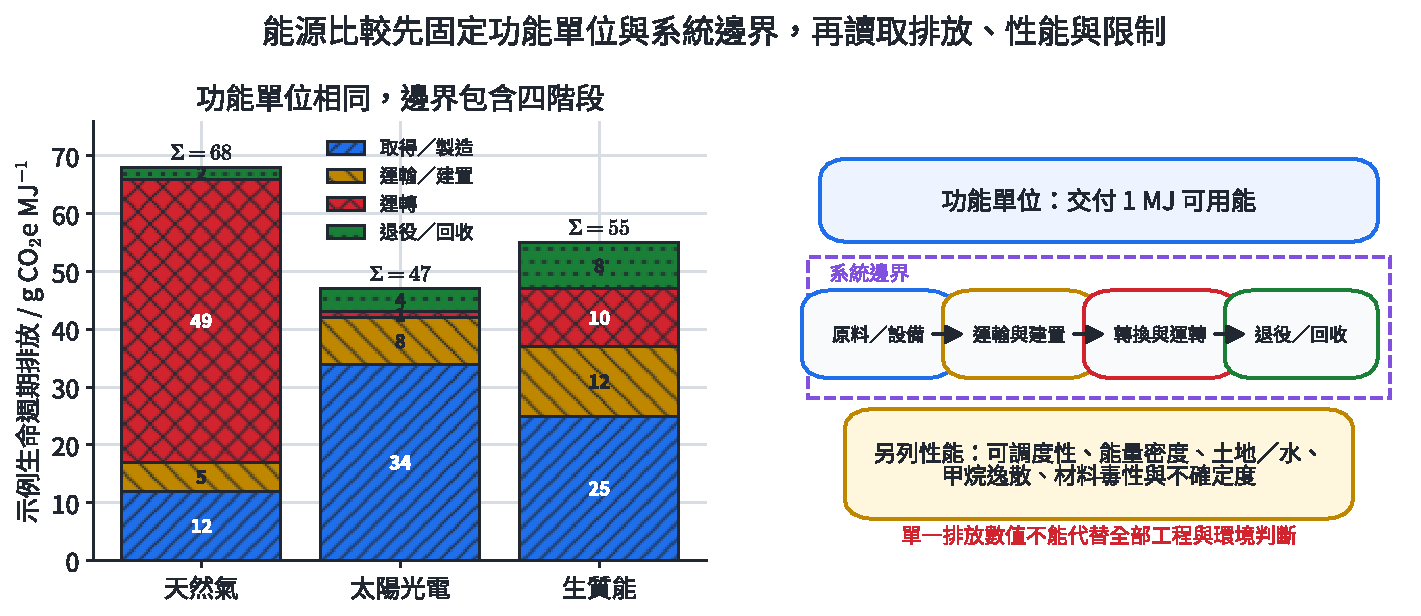
\includegraphics[width=0.99\linewidth,height=\textheight,keepaspectratio,alt={圖 13｜左圖以色彩、線紋、分段數值與總和標示三種能源的四個生命週期階段；右圖固定功能單位與系統邊界。}]{assets/選化V-2-能源生命週期邊界.pdf}
\caption{圖 13｜左圖以色彩、線紋、分段數值與總和標示三種能源的四個生命週期階段；右圖固定功能單位與系統邊界。}
\end{figure}

圖 13 的數值是示例資料，用來練習讀圖：太陽光電的運轉階段低，製造與建置占比較高；天然氣的運轉階段占比高；生質能結果取決於原料與土地邊界。圖中總量只代表此資料集，不可取代特定地區、技術與年份的正式盤查。

\begin{HandoutWorkedExample}

\subsection{示範 26｜由堆疊資料比較總量與熱點}\label{ux793aux7bc4-26ux7531ux5806ux758aux8cc7ux6599ux6bd4ux8f03ux7e3dux91cfux8207ux71b1ux9ede}

圖 13 中天然氣四階段為 \(12,5,49,2\)，合計 \(68\ \mathrm{g\ CO_2e\ MJ^{-1}}\)；太陽光電為 \(34,8,1,4\)，合計 \(47\)；生質能為 \(25,12,10,8\)，合計 \(55\)。在此功能單位與邊界下，太陽光電總值最低，其熱點是設備製造；天然氣的熱點是運轉燃燒。改善策略應對準各自熱點。

\end{HandoutWorkedExample}

\begin{HandoutWorkedExample}

\subsection{示範 27｜加入甲烷逸散後修正比較}\label{ux793aux7bc4-27ux52a0ux5165ux7532ux70f7ux9038ux6563ux5f8cux4feeux6b63ux6bd4ux8f03}

某天然氣系統原生命週期排放為 \(68\ \mathrm{g\ CO_2e\ MJ^{-1}}\)，後來量測上游逸散使額外氣候影響為 \(14\ \mathrm{g\ CO_2e\ MJ^{-1}}\)。修正值為 \(82\ \mathrm{g\ CO_2e\ MJ^{-1}}\)，增加比例

\[
\frac{14}{68}\times100\%=20.6\%.
\]

「CO₂e」換算會依採用的氣候時間尺度與係數改變，報告需列出換算基準；化學計量的燃燒 \(CO_2\) 與逸散甲烷要分項保留。

\end{HandoutWorkedExample}

\subsection{理解用／可略讀：鹽度梯度能與滲透壓}\label{ux7406ux89e3ux7528ux53efux7565ux8b80ux9e7dux5ea6ux68afux5ea6ux80fdux8207ux6ef2ux900fux58d3}

淡水與海水由只允許水通過的半透膜隔開時，化學勢差驅動水向高溶質側移動。理想稀溶液的滲透壓近似

\[
\pi=iMRT.
\]

若利用壓力延遲滲透或電滲析取得能量，實際輸出會低於理論混合自由能，因膜阻力、濃差極化、泵耗與生物附著造成損失。能量來源是兩股水混合時的自由能下降。

\begin{HandoutWorkedExample}

\subsection{示範 28｜估算理想鹽溶液滲透壓}\label{ux793aux7bc4-28ux4f30ux7b97ux7406ux60f3ux9e7dux6eb6ux6db2ux6ef2ux900fux58d3}

以 \(0.50\ \mathrm M\) NaCl、\(25^\circ\mathrm C\)，理想完全解離取 \(i=2.0\)，\(R=0.0821\ \mathrm{L\ atm\ mol^{-1}\ K^{-1}}\)：

\[
\pi=(2.0)(0.50)(0.0821)(298)=24.5\ \mathrm{atm}.
\]

海水離子濃度高，非理想性顯著，此值是量級估算；工程設計需用活度與膜性能資料。

\end{HandoutWorkedExample}

\subsection{練習 7}\label{ux7df4ux7fd2-7}

\begin{enumerate}
\def\labelenumi{\arabic{enumi}.}
\tightlist
\item
  依甲烷燃燒式，\(4.00\) mol \(CH_4\) 完全燃燒需多少 mol \(O_2\)，生成多少 g \(CO_2\)？
\item
  燃料直接排放強度為 \(50.0\ \mathrm{g\ CO_2\ MJ^{-1}}\)，發電效率 \(40.0\%\)；求每 MJ 電力的直接排放。
\item
  某能源四階段排放為 \(18,7,3,5\ \mathrm{g\ CO_2e\ MJ^{-1}}\)。求總量與占比最大的階段。
\item
  方案 A 生命週期排放 \(45\ \mathrm{g\ CO_2e\ MJ^{-1}}\)、可隨時調度；方案 B 為 \(25\)、輸出受天候影響。列出作電力系統比較時還需的兩項資料。
\item
  \(0.20\ \mathrm M\) 理想 \(CaCl_2\) 溶液在 \(298\) K，完全解離取 \(i=3\)；用 \(R=0.0821\ \mathrm{L\ atm\ mol^{-1}\ K^{-1}}\) 估算滲透壓。
\end{enumerate}

\subsection{練習 7 解析}\label{ux7df4ux7fd2-7-ux89e3ux6790}

\begin{enumerate}
\def\labelenumi{\arabic{enumi}.}
\tightlist
\item
  係數比 \(CH_4:O_2:CO_2=1:2:1\)，需 \(8.00\) mol \(O_2\)，生成 \(4.00(44.0)=176\) g \(CO_2\)。
\item
  交付 \(1\) MJ 電力需 \(1/0.400=2.50\) MJ 燃料，排放 \(50.0(2.50)=125\ \mathrm{g\ CO_2}\) 每 MJ 電力。
\item
  總量 \(18+7+3+5=33\ \mathrm{g\ CO_2e\ MJ^{-1}}\)；原料取得／製造的 \(18\) 最大，占 \(18/33=54.5\%\)。
\item
  可加入儲能或備援需求、容量因數、建置時間、電網位置、土地／水使用、設備壽命與成本；任列兩項且維持相同供電可靠度功能。
\item
  \(\pi=iMRT=(3)(0.20)(0.0821)(298)=14.7\ \mathrm{atm}\)。這是假設完全解離與理想溶液的估值。
\end{enumerate}

能源化學把燃料反應、材料製造與污染控制放在同一功能單位下。直接排放、生命週期排放、可靠度與資源限制需分欄報告；單一總分會隱藏重要取捨。

\section{8. 章末分層題}\label{ux7ae0ux672bux5206ux5c64ux984c}

\subsection{基礎與機制題 1--6}\label{ux57faux790eux8207ux6a5fux5236ux984c-16}

\begin{enumerate}
\def\labelenumi{\arabic{enumi}.}
\tightlist
\item
  反應 \(CaO+CO_2\rightarrow CaCO_3\) 以 \(CaCO_3\) 為目標產物。求原子經濟率；若理論產量 \(100\) g、實得 \(86\) g，再求產率。
\item
  某臭氧模型預測四週柱量為 \(300,294,288,282\) DU，觀測為 \(301,293,284,274\) DU。（a）求各週殘差「觀測－預測」；（b）判斷是否需檢查模型；（c）把第四週 \(274\) DU 換成標準狀況臭氧厚度。
\item
  水樣占稀釋瓶 \(15.0\%\)，DO 由 \(8.8\) 降至 \(6.5\ \mathrm{mg\ L^{-1}}\)。求 \(BOD_5\)，並寫出兩項方法條件。
\item
  湖水增肥試驗葉綠素 a 為：對照 \(4.0\)、加 N \(4.8\)、加 P \(18.0\)、加 N+P \(23.0\ \mu\mathrm{g\,L^{-1}}\)。（a）判斷主要限制營養鹽；（b）寫出由營養鹽到低氧的因果鏈。
\item
  某污染物濃度：水 \(5.0\times10^{-5}\ \mathrm{mg\ L^{-1}}\)、浮游生物 \(0.010\ \mathrm{mg\ kg^{-1}}\)、小魚 \(0.20\ \mathrm{mg\ kg^{-1}}\)、大型魚 \(0.80\ \mathrm{mg\ kg^{-1}}\)。求水到浮游生物的 BCF 與小魚到大型魚的 BMF。
\item
  水樣依序經（甲）濾紙過濾、（乙）明礬混凝---沉降---過濾。原水、甲、乙濁度為 \(62,25,4\) NTU，導電度為 \(510,500,485\ \mu\mathrm{S\,cm^{-1}}\)。（a）說明兩步主要移除的物質形態；（b）是否能由此判定乙可飲用？（c）列出雷射與未知水樣各一項安全控制。
\end{enumerate}

\subsection{資料與定量題 7--12}\label{ux8cc7ux6599ux8207ux5b9aux91cfux984c-712}

\begin{enumerate}
\def\labelenumi{\arabic{enumi}.}
\setcounter{enumi}{6}
\tightlist
\item
  午後 \(NO_2\) 受光解後形成近地面臭氧。（a）寫出兩步反應；（b）指出 \(O\) 的角色；（c）說明 VOC 為何可能促使臭氧累積。
\item
  題目提供 PM₂.₅ 斷點 \(25\to I=50\)、\(50\to I=100\)，測得 \(40\)；O₃ 分指標為 \(76\)。（a）求 PM₂.₅ 分指標；（b）求 AQI 與主導污染物；（c）說明 AQI 為何不等於個人吸入劑量。
\item
  某河流量 \(1.8\times10^8\ \mathrm{L\ day^{-1}}\)，總磷濃度 \(0.080\ \mathrm{mg\ L^{-1}}\)。（a）求每日總磷負荷 kg day\(^{-1}\)；（b）若濃度降低 \(25\%\)、流量增加 \(20\%\)，新負荷為原來幾倍？
\item
  一農田每季輸入 \(150\) kg N ha\(^{-1}\)；收穫帶走 \(82\)、氨揮發 \(16\)、反硝化 \(22\)、土壤增加 \(12\)。（a）求淋洗／逕流；（b）若排水量 \(2.0\times10^6\) L ha\(^{-1}\)，全部水輸出視為硝酸鹽氮，求平均濃度 mg N L\(^{-1}\)；（c）指出此平均模型的一項限制。
\item
  某燃料近似純甲烷。機組效率 \(50.0\%\)，甲烷每 mol 放熱 \(890\) kJ。（a）交付 \(1.00\) MJ 電力需幾 mol \(CH_4\)？（b）生成幾 g \(CO_2\)？（c）此結果未含哪些生命週期項目？任列兩項。
\item
  三種供能方案以相同功能單位得到下表：
\end{enumerate}

{\def\LTcaptype{none} % do not increment counter
\begin{longtable}[]{@{}lrrrrl@{}}
\toprule\noalign{}
方案 & 製造 & 運輸建置 & 運轉 & 退役 & 可調度性 \\
\midrule\noalign{}
\endhead
\bottomrule\noalign{}
\endlastfoot
A & 20 & 5 & 45 & 3 & 高 \\
B & 35 & 8 & 2 & 5 & 低 \\
C & 24 & 10 & 12 & 6 & 中 \\
\end{longtable}
}

單位皆為 \(\mathrm{g\ CO_2e\ MJ^{-1}}\)。（a）求三方案總量；（b）指出各自排放熱點；（c）若任務要求連續供電，還需加入哪一類系統資料？

\subsection{跨節整合題 13--16}\label{ux8de8ux7bc0ux6574ux5408ux984c-1316}

\begin{enumerate}
\def\labelenumi{\arabic{enumi}.}
\setcounter{enumi}{12}
\tightlist
\item
  某工廠比較兩條製造 \(100\) kg 產品的路線。甲：原子經濟率 \(80\%\)、產率 \(75\%\)、廢棄物 \(160\) kg、用能 \(900\) MJ；乙：原子經濟率 \(65\%\)、產率 \(92\%\)、廢棄物 \(95\) kg、用能 \(1300\) MJ。能源生命週期排放強度皆為 \(55\ \mathrm{g\ CO_2e\ MJ^{-1}}\)。（a）求兩路線 E-factor；（b）求能源相關排放 kg CO₂e；（c）分別指出哪條路線在原子經濟率、產率、廢棄物與能源排放較佳；（d）提出一項可檢驗的乙路線改善方案與所需資料。
\item
  一座水庫上游處理廠排水量 \(3.0\times10^6\ \mathrm{L\ day^{-1}}\)，硝酸鹽氮 \(9.0\ \mathrm{mg\ L^{-1}}\)，原水 \(BOD_5=20\ \mathrm{mg\ L^{-1}}\)。改善後氮濃度降為 \(5.0\ \mathrm{mg\ L^{-1}}\)，\(BOD_5\) 降為 \(8.0\ \mathrm{mg\ L^{-1}}\)，流量不變。（a）求每日氮負荷減少量；（b）求 BOD 氧當量負荷減少量；（c）用氮、藻類、分解與 DO 串成改善機制；（d）列出兩項水庫監測資料，以檢驗機制而非只比較出流水。
\item
  都市監測資料顯示：上午 8 時 NO \(80\) ppb、O₃ \(15\) ppb；下午 2 時 NO \(18\) ppb、O₃ \(74\) ppb。模型預測下午 O₃ 為 \(58\) ppb。題目斷點給 O₃：\(50\to I=50\)、\(70\to I=100\)、\(85\to I=150\)。（a）說明早晚資料符合的反應機制；（b）求下午 O₃ 分指標；（c）求模型殘差；（d）提出兩個可量測變數以判斷偏差來自 VOC 化學或大氣傳輸。
\item
  農場每季施入 \(200\) kg N；作物帶走 \(110\)、土壤累積 \(20\)、氨揮發 \(18\)、反硝化 \(22\)，其餘進入排水。農場另把廢棄生質物厭氧消化，產生 \(800\) mol \(CH_4\)，其中 \(3.0\%\) 逸散，其餘完全燃燒；每 mol \(CH_4\) 提供 \(890\) kJ 熱，設備回收效率 \(40\%\)。（a）求氮的水輸出；（b）求可利用熱能 MJ；（c）求燃燒生成 \(CO_2\) 的質量；（d）說明這套系統同時改善與新增的環境議題，並列兩項必要監測。
\end{enumerate}

\section{9. 章末題完整解析}\label{ux7ae0ux672bux984cux5b8cux6574ux89e3ux6790}

\begin{enumerate}
\def\labelenumi{\arabic{enumi}.}
\item
  平衡式只有一個產物，反應物所有原子都進入 \(CaCO_3\)，原子經濟率 \(100\%\)。產率 \(=86/100\times100\%=86\%\)。前者由計量式決定，後者由實際產量決定。
\item
  （a）殘差依序為 \(+1,-1,-4,-8\) DU。（b）後兩週持續為負且幅度增大，觀測下降快於模型，需檢查光照、活性氯、輸送或儀器校正，並以新資料比較修正模型。（c）\(274(0.01)=2.74\) mm。DU 為整柱量，不是單一高度濃度。
\item
  由稀釋水樣的溶氧下降量換算原水樣：
  \[
  BOD_5=\frac{8.8-6.5}{0.150}=15.3\ \mathrm{mg\ L^{-1}}.
  \]
  方法條件可列五日、規定溫度（常用 \(20^\circ\mathrm C\)）、暗處、適當稀釋、種菌與空白修正；任兩項。
\item
  （a）加 P 由 \(4.0\) 增至 \(18.0\)，遠大於加 N，P 是此條件下主要限制營養鹽；N+P 更高，顯示解除 P 限制後 N 或交互作用仍有影響。（b）N、P 輸入 → 藻類增生 → 遮光與死亡 → 分解者耗氧 → 底層低氧。此結論需保留季節與水層尺度。
\item
  水到浮游生物：\(BCF=0.010/(5.0\times10^{-5})=200\ \mathrm{L\ kg^{-1}}\)。小魚到大型魚：\(BMF=0.80/0.20=4.0\)。第一個是介質---生物濃縮，第二個是營養階層放大。
\item
  （a）濾紙先移除較大懸浮粒子；明礬形成 \(Al(OH)_3\) 絮體，吸附／網捕較小膠體，再沉降與過濾。（b）不能；尚未檢測病原、溶解離子、有機毒物與消毒效果。導電度仍高也支持溶解離子大多留存。（c）雷射固定向下照射且避開人眼與反光面；未知水樣戴護目鏡、手套並禁止入口，任各一項。
\item
  （a）\(NO_2+h\nu\rightarrow NO+O\)；\(O+O_2+M\rightarrow O_3+M\)。（b）O 在第一步生成、第二步消耗，是中間體。（c）VOC 氧化自由基可把 NO 轉回 \(NO_2\)，卻不必同時消耗 \(O_3\)，使光解---生成循環持續並讓臭氧累積。
\item
  （a）
  \[
  I_{PM}=50+\frac{100-50}{50-25}(40-25)=80.
  \]
  （b）\(AQI=\max(80,76)=80\)，主導污染物為 PM₂.₅。（c）AQI 是監測站、特定平均時間的標準化指標；個人劑量還受停留時間、位置、呼吸率、室內滲透與防護影響。
\item
  （a）
  \[
  L=(0.080)(1.8\times10^8)=1.44\times10^7\ \mathrm{mg\ day^{-1}}
  =14.4\ \mathrm{kg\ day^{-1}}.
  \]
  （b）新濃度為 \(0.75C\)、新流量為 \(1.20Q\)，新負荷比 \(=0.75(1.20)=0.90\)；負荷只降 \(10\%\)。
\item
  （a）水輸出 \(=150-82-16-22-12=18\ \mathrm{kg\ N\ ha^{-1}}\)。（b）\(18\) kg \(=1.8\times10^7\) mg，除以 \(2.0\times10^6\) L 得 \(9.0\ \mathrm{mg\ N\ L^{-1}}\)。（c）平均模型忽略暴雨尖峰、其他水路、不同氮物種與空間差異，任列一項。
\item
  （a）交付 \(1.00\) MJ 電力需熱量 \(1.00/0.500=2.00\) MJ；甲烷量 \(=2000/890=2.25\) mol。（b）每 mol 生成一 mol \(CO_2\)，質量 \(2.25(44.0)=98.9\) g。（c）未含開採、製氣、壓縮輸送、甲烷逸散、設備製造與退役；任列兩項。
\item
  （a）A：\(20+5+45+3=73\)；B：\(35+8+2+5=50\)；C：\(24+10+12+6=52\ \mathrm{g\ CO_2e\ MJ^{-1}}\)。（b）A 熱點是運轉 \(45\)；B 是製造 \(35\)；C 是製造 \(24\)。（c）還需容量因數、時序輸出、儲能與備援效率／排放、電網限制或需求曲線，並以相同可靠供電功能比較。
\item
  （a）\(E_{\text{甲}}=160/100=1.60\)；\(E_{\text{乙}}=95/100=0.95\)。（b）甲：\(900(55)=49500\) g \(=49.5\) kg CO₂e；乙：\(1300(55)=71500\) g \(=71.5\) kg CO₂e。（c）甲的原子經濟率較高且能源排放較低；乙的產率較高且 E-factor／廢棄物較低。（d）例如檢驗乙是否能以催化劑降溫或縮短分離：量測相同純度與產率下的反應溫度、時間、分離能耗、催化劑壽命與新增廢棄物。改善需以同一 \(100\) kg 產品功能單位重算。
\item
  （a）氮濃度下降 \(4.0\ \mathrm{mg\ L^{-1}}\)：
  \[
  \Delta L_N=(4.0)(3.0\times10^6)=1.2\times10^7\ \mathrm{mg}=12\ \mathrm{kg\ N\ day^{-1}}.
  \]
  （b）BOD 氧當量下降 \(12\ \mathrm{mg\ L^{-1}}\)：\(36\ \mathrm{kg\ O_2\ day^{-1}}\)。（c）可利用氮輸入下降 → 藻類增生壓力下降；有機負荷下降 → 分解耗氧下降；兩者共同提高底層維持 DO 的可能性。（d）監測水庫 N／P 物種、葉綠素 a、透明度、分層溫度、不同深度與日夜 DO、流入流量；至少兩項且需包含反應鏈中間或結果量。
\item
  （a）早晨交通排放使 NO 高；日照下 \(NO_2\) 光解並在 VOC 自由基作用下形成、累積 \(O_3\)，下午 NO 降而 O₃ 升，符合一次前驅物轉成二次污染物。（b）\(74\) 位於 \(70\)--\(85\) 對應 \(100\)--\(150\)：
  \[
  I=100+\frac{50}{15}(74-70)=113.3\approx113.
  \]
  （c）殘差 \(=74-58=+16\) ppb，模型低估。（d）量測 VOC 組成／反應性與 \(NO_x\) 可檢查化學；量測風向風速、混合層高度或上風處 O₃ 可檢查傳輸，兩類各一較有診斷力。
\item
  （a）水輸出 \(=200-110-20-18-22=30\) kg N。（b）燃燒甲烷 \(=800(0.970)=776\) mol；化學熱 \(=776(890)=690640\) kJ，回收 \(40\%\) 得 \(276256\) kJ \(=276\) MJ。（c）燃燒生成 \(776\) mol \(CO_2\)，質量 \(=776(44.0)=34.1\) kg。（d）改善面包含回收廢棄生質物能量、減少未處理有機物與替代部分外購燃料；新增或保留議題包含 \(3\%\) 甲烷逸散、燃燒 \(CO_2\)、氮水輸出及消化液管理。必要監測可列甲烷產量與逸散率、排水氮物種與流量、消化液養分、設備效率、NOₓ 或生命週期替代量；任兩項並連到上述機制。
\end{enumerate}

\section{10. 核心整理}\label{ux6838ux5fc3ux6574ux7406}

\begin{itemize}
\tightlist
\item
  原子經濟率看平衡式的理論原子去向；產率看實際／理論產物；E-factor 看指定邊界內每單位產品的廢棄物。
\item
  模型需附目的、尺度、假設、可觀測量與不確定度。殘差若持續同方向增大，表示需檢查機制、參數或量測校正。
\item
  平流層臭氧由氧的光化學循環維持；氯自由基在催化循環中再生。DU 是垂直整柱總量，\(1\) DU 對應標準狀況 \(0.01\) mm 臭氧。
\item
  DO 是當下溶氧濃度；\(BOD_5\) 是規定條件下五日的生物耗氧量；COD 是規定化學氧化法的氧當量。方法條件屬定義的一部分。
\item
  優養化的機制是營養鹽輸入、藻增生、死亡分解與低氧；限制營養鹽需用控制實驗與當地資料判定。
\item
  生物累積比較生物與介質；生物放大比較捕食者與食物。濃度需附介質、組織、單位與採樣尺度。
\item
  濁度量散射，導電度量離子整體導電能力。過濾主要移除大顆粒；混凝形成絮體移除膠體；飲用水製程仍需依用途完成消毒。
\item
  一次污染物直接排放，二次污染物在大氣反應形成。AQI 先把各濃度換成分指標，再取最大值；個人暴露還需時間與位置。
\item
  物料平衡先固定控制體與時間；污染負荷 \(L=CQ\)。濃度、總量與通量回答不同問題。
\item
  硝化是需氧的氧化過程並產生酸度；反硝化在缺氧與有電子供體時把硝酸根還原。農田氮收支需保留作物、氣體、土壤與水路徑。
\item
  能源比較固定功能單位與生命週期邊界，分列直接排放、上游逸散、製造、運輸、退役、可靠度與資源限制。
\end{itemize}


\end{document}
